\documentclass[envcountsect,dvips]{beamer}

\setbeamertemplate{background canvas}[vertical shading][bottom=yellow!20,top=blue!10]
%\usetheme{Darmstadt}
\usetheme{Warsaw}
%\usefonttheme[onlysmall]{structurebold}

\usepackage{natbib}
\usepackage{bibentry}
\bibliographystyle{apalike}
\usepackage{chngcntr}

\usepackage[utf8]{inputenc}
\usepackage{default}
\usepackage{amsmath}
\usepackage{amsfonts}
\usepackage{amssymb}

\usepackage{graphicx}
\usepackage{caption}
\usepackage{subcaption}

\usepackage{color,xcolor,ucs}% para textcolor



%%%%%%%%%%%%%%%%%%%%%%%%%%%%%%%%%%%%%%%%%%%%%%%%%%%%%%%%%%%%%%%%%%%%%%%%%%
\begin{document}

\title[Transistores bipolares:   ] % (optional, only for long titles)
{Transistores bipolares:}
\subtitle{Construção, caraterísticas e aplicações}
\author[Fernando] % (optional, for multiple authors)
{Fernando Pujaico Rivera\inst{1}}
\institute[Universidade Federal de Lavras] % (optional)
{
  \inst{1}%
  Universidade Federal de Lavras
}
\date[2016] % (optional)
{Aula-1 2016}
\subject{Computer Science}
\frame{\titlepage}

%%%%%%%%%%%%%%%%%%%%%%%%%%%%%%%%%%%%%%%%%%%%%%%%%%%%%%%%%%%%%%%%%%%%%%%%%%%%%%%%
%%%%%%%%%%%%%%%%%%%%%%%%%%%%%%%%%%%%%%%%%%%%%%%%%%%%%%%%%%%%%%%%%%%%%%%%%%%%%%%%
%%%%%%%%%%%%%%%%%%%%%%%%%%%%%%%%%%%%%%%%%%%%%%%%%%%%%%%%%%%%%%%%%%%%%%%%%%%%%%%%
\section{Construção}
%%https://www.youtube.com/watch?v=X0XscX9ugp0


\begin{frame}{Descrição simples do transistor - Bipolar junction transistor \cite{boylestaddispositivos} }
\begin{figure}
\centering
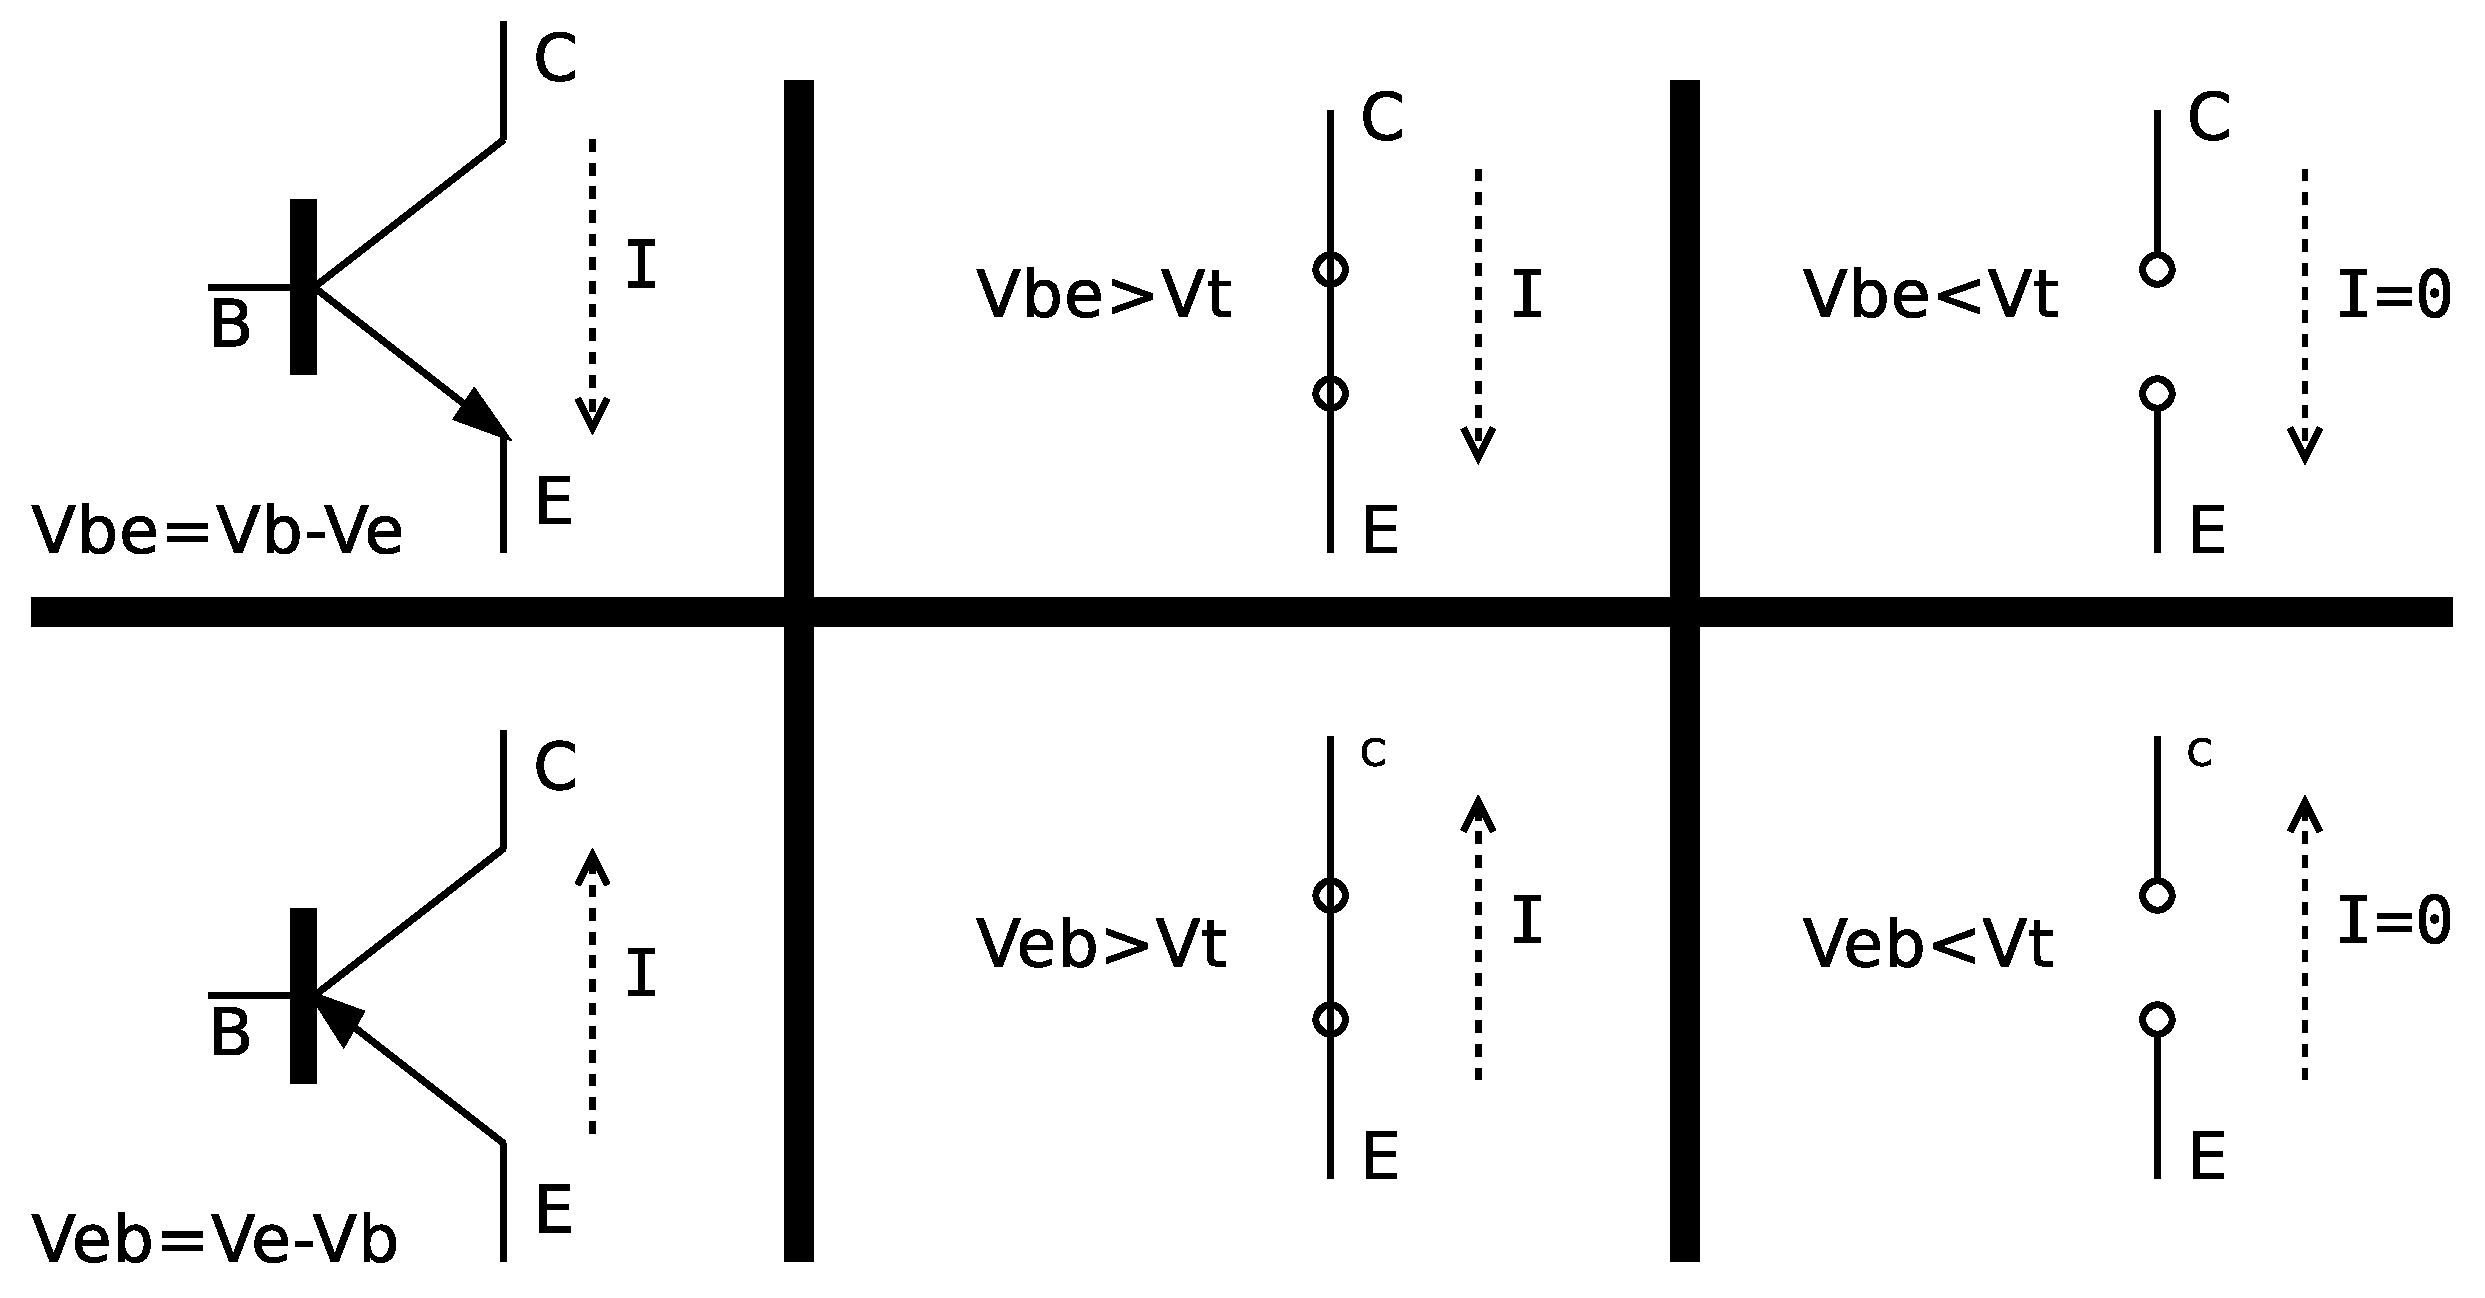
\includegraphics[width=9cm]{images/simple.eps}
\caption{Descrição  do BJT em saturação}
\label{fig:simples}
\end{figure}
\end{frame}


\begin{frame}{Semicondutor  }
\begin{figure}
\centering
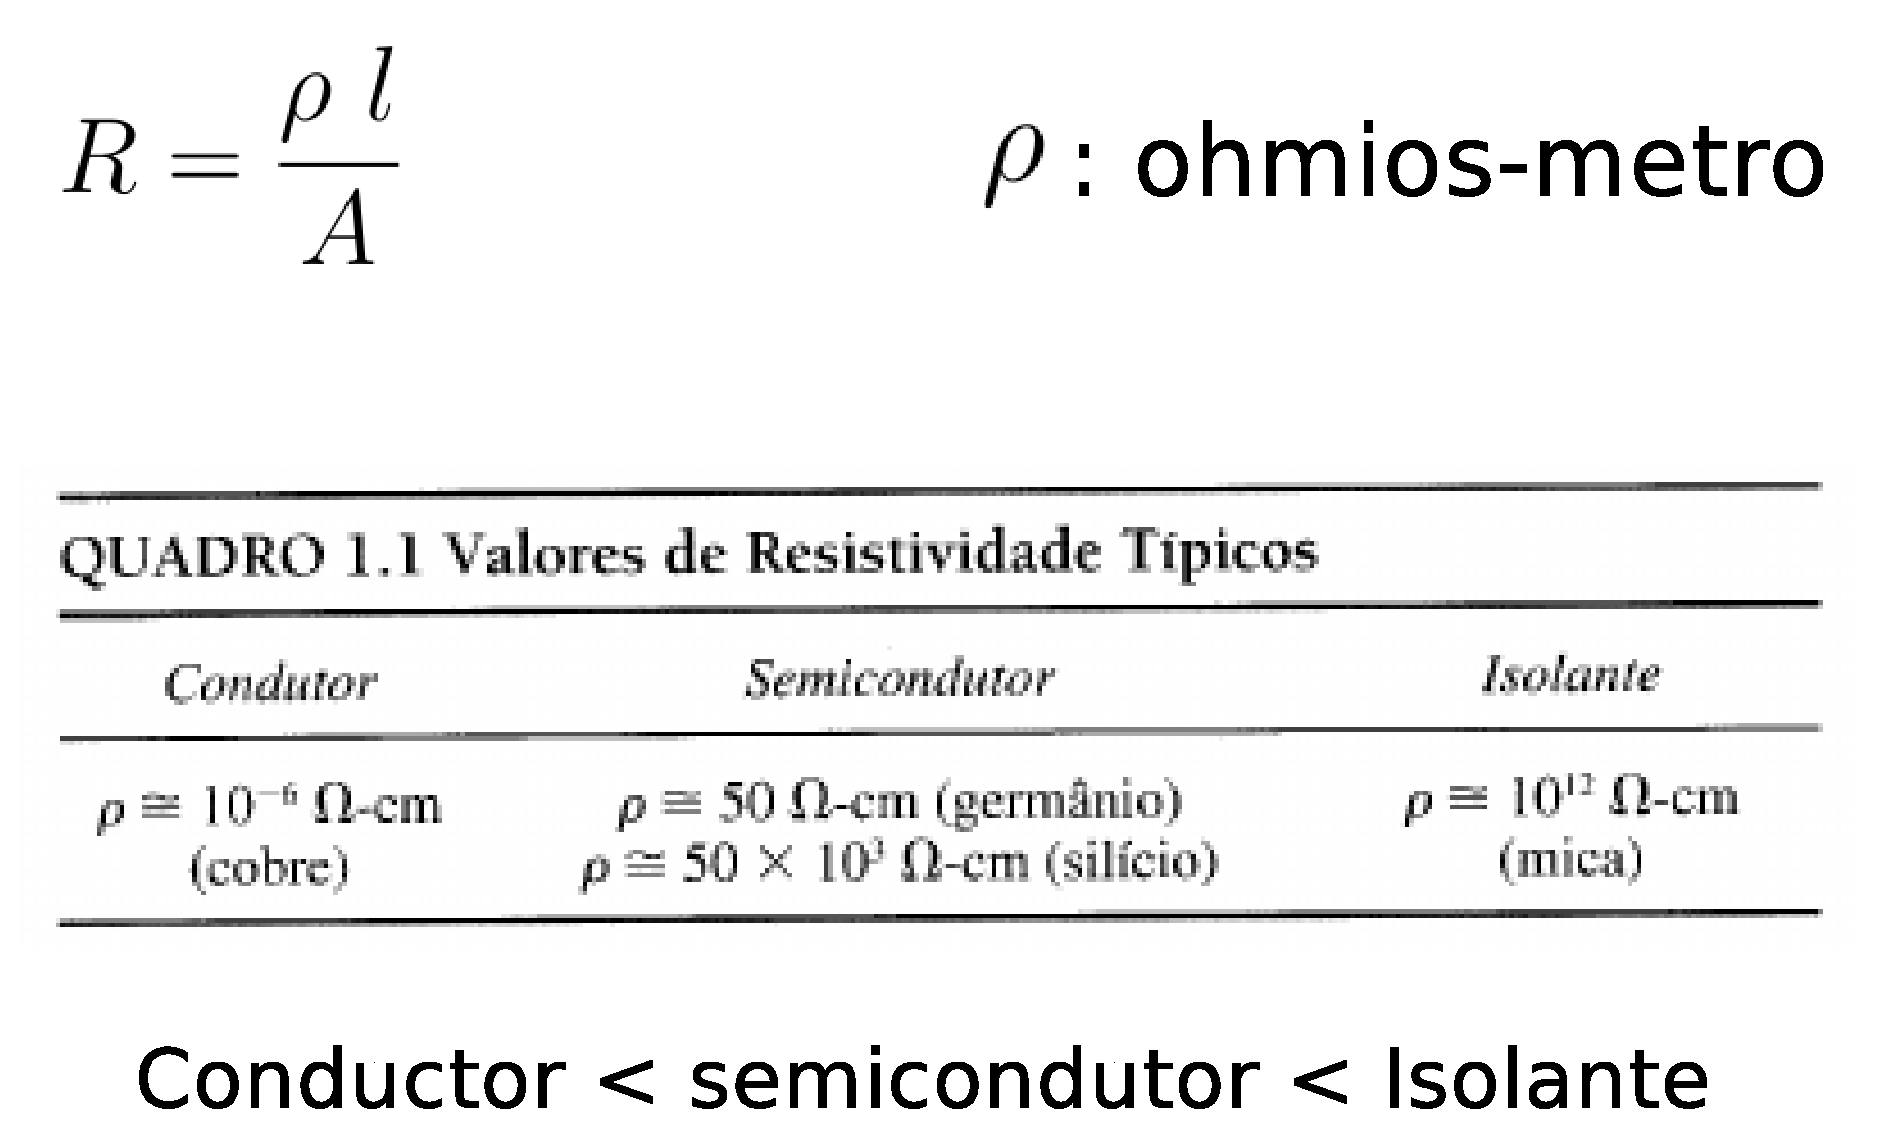
\includegraphics[width=9cm]{images/conductor.eps}
\caption{Resistência ao fluxo de carga}
\label{fig:conductor}
\end{figure}
\end{frame}

\begin{frame}{Materiais condutores   }
\begin{figure}
\centering
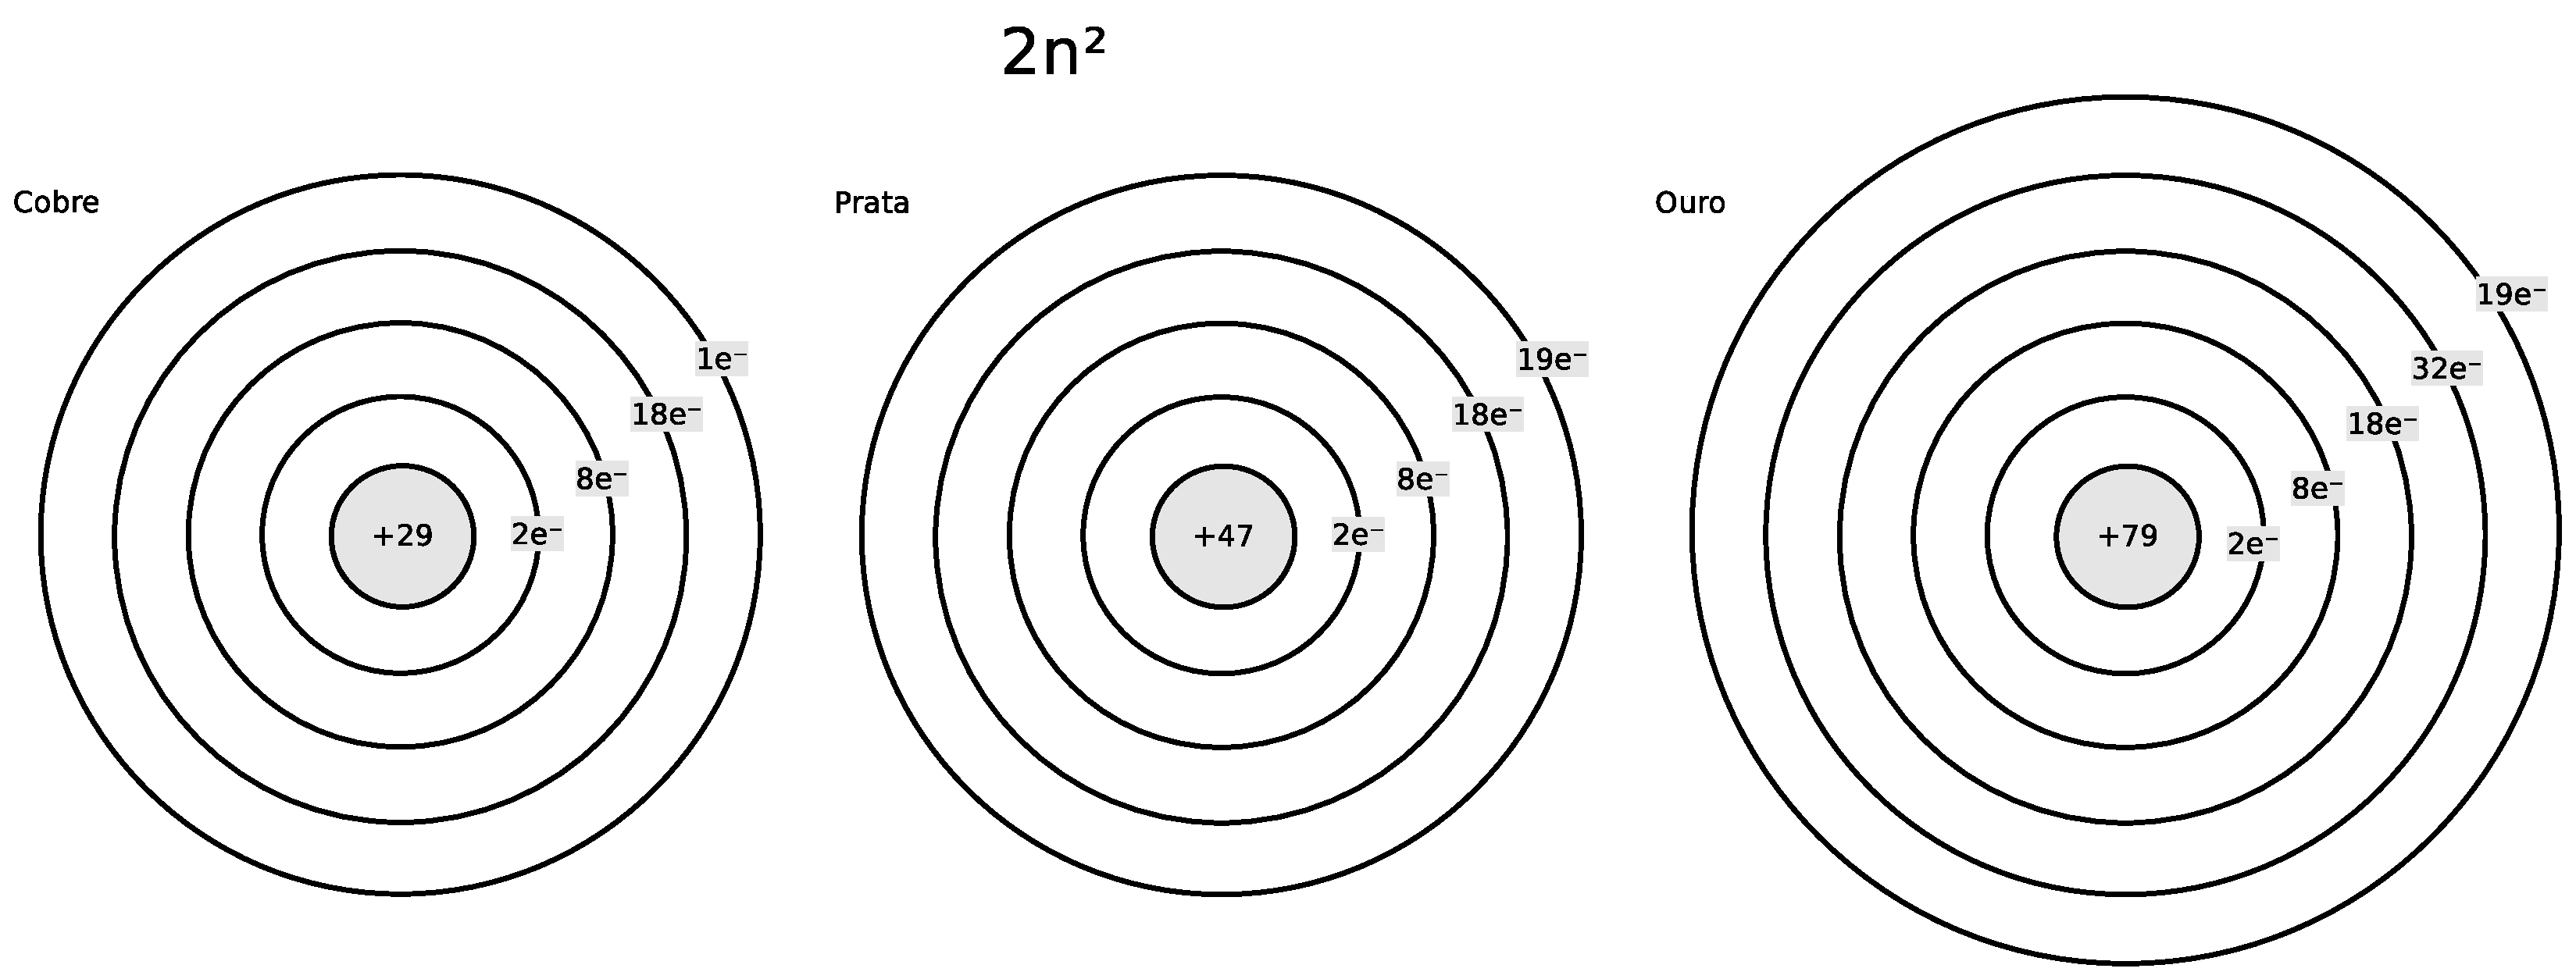
\includegraphics[width=10cm]{images/cobre.eps}
\caption{Elétrons nas camadas e camadas de valência}
\label{fig:dopagem}
\end{figure}
\end{frame}

\begin{frame}{Materiais semicondutores}
\begin{figure}
\centering
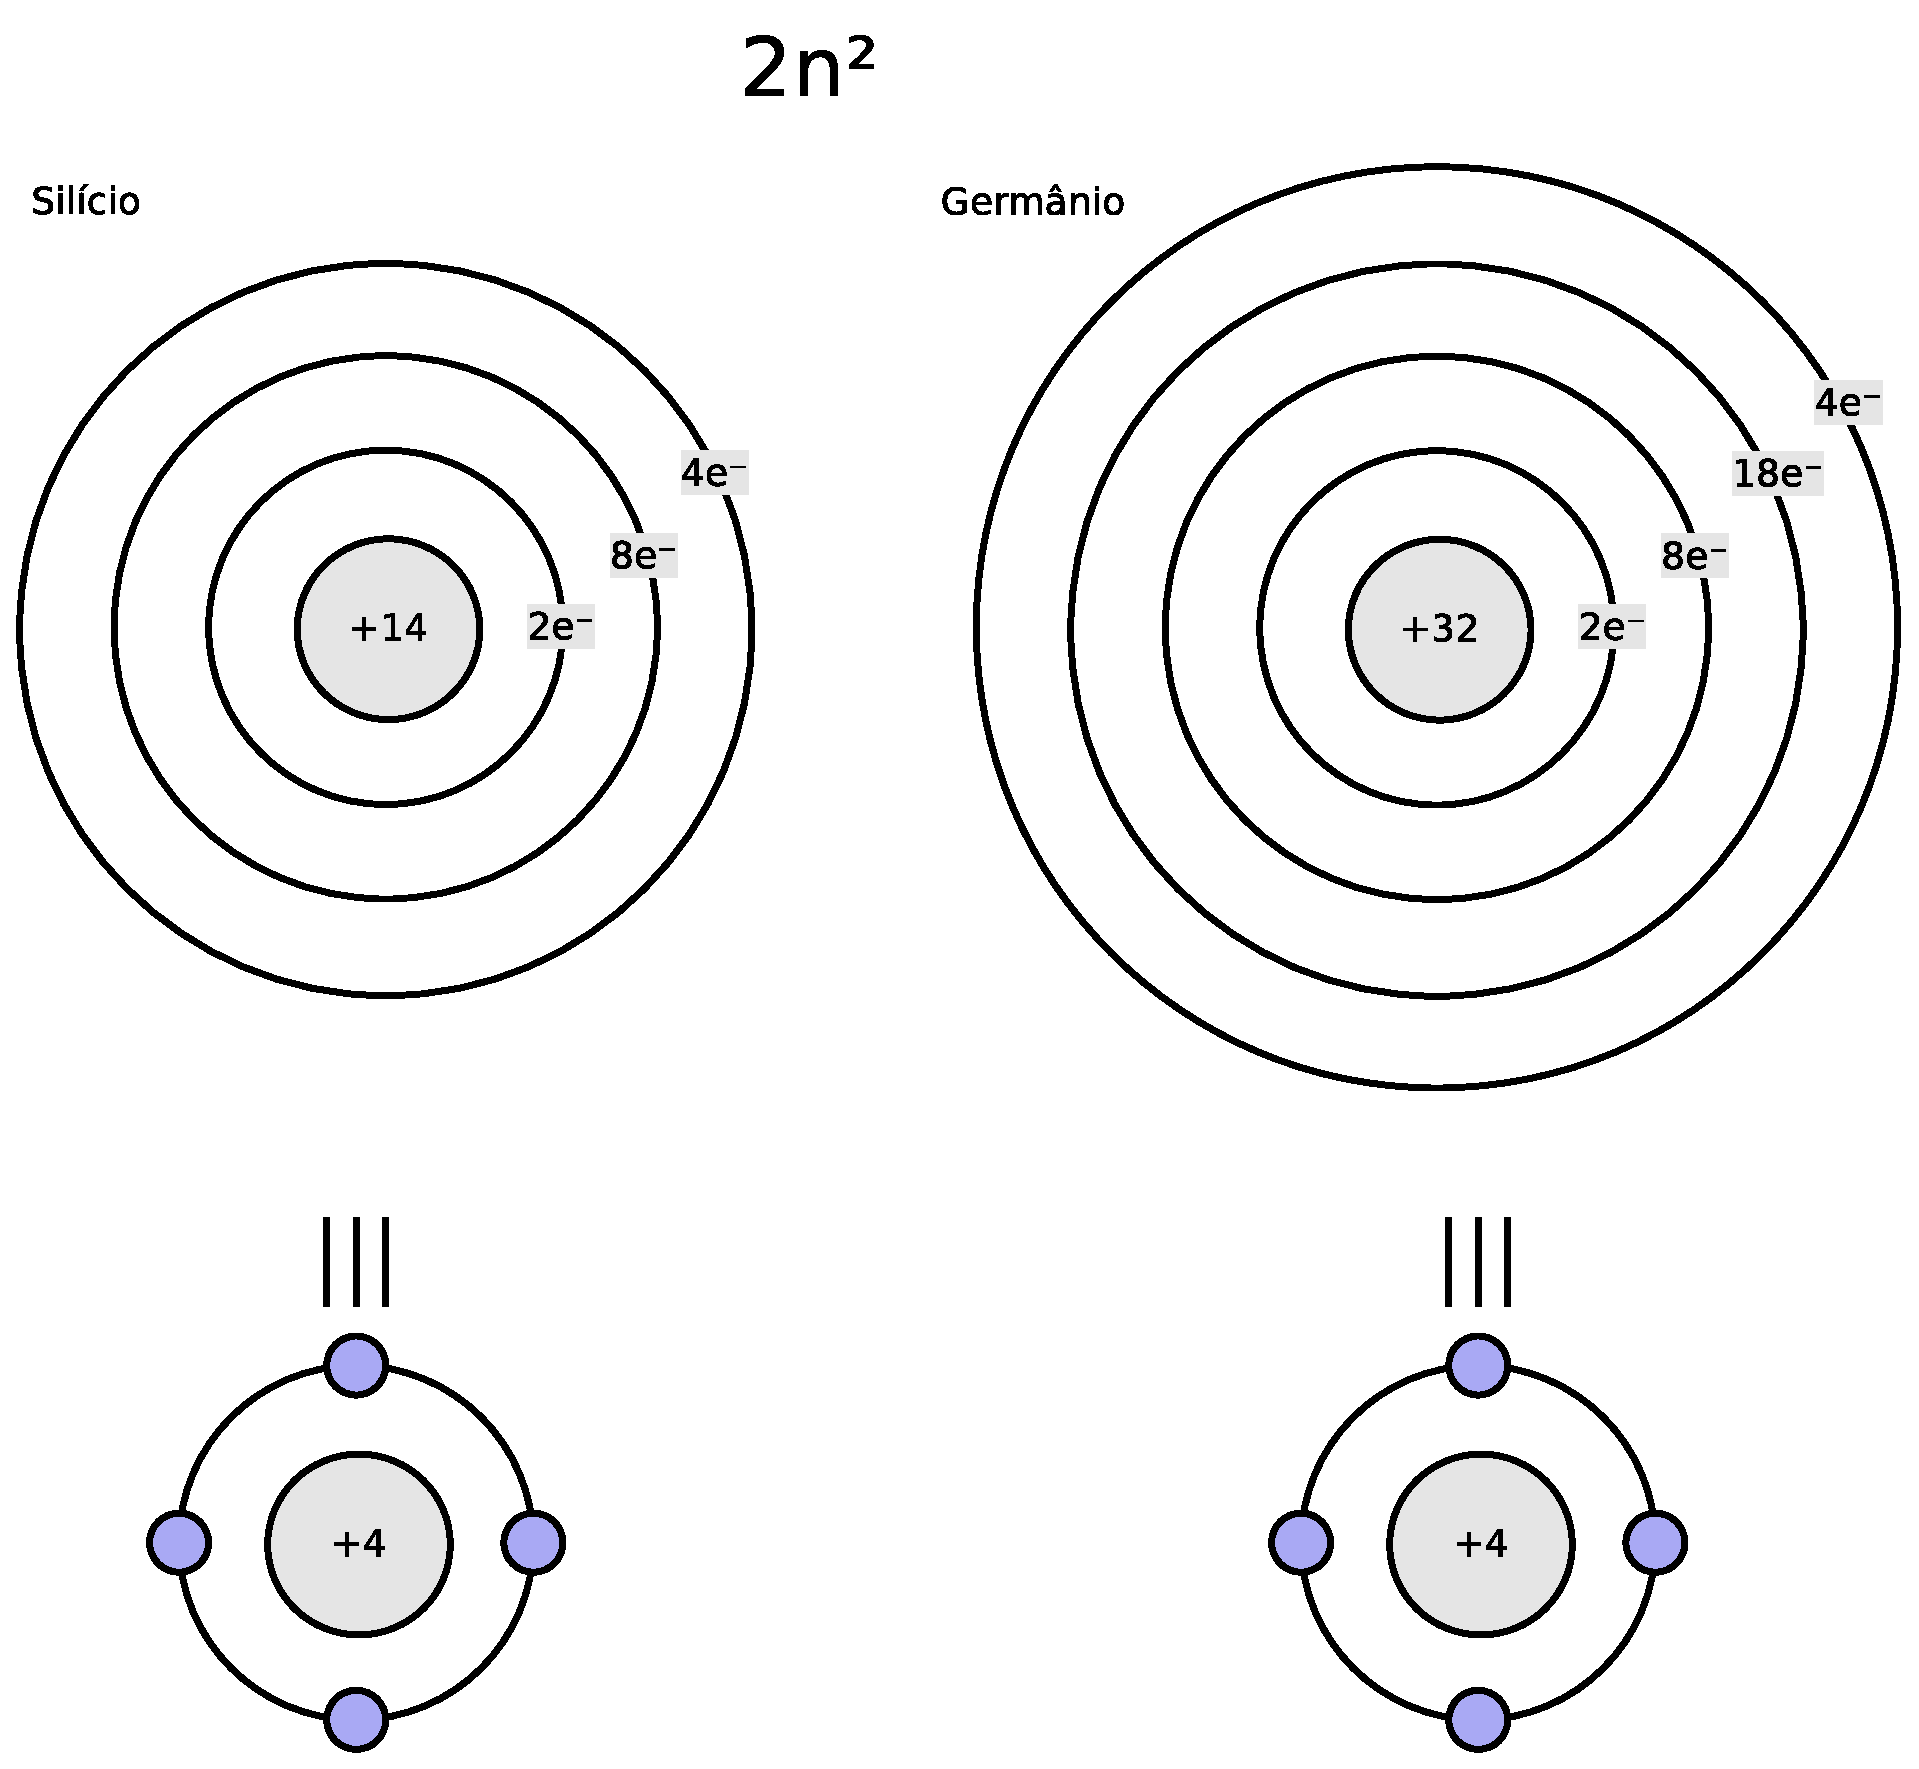
\includegraphics[width=5cm]{images/sige.eps}
\caption{Elétrons nas camadas e camadas de valência}
\label{fig:sige}
\end{figure}
\end{frame}

\begin{frame}{Semicondutor intrínseco}
\begin{figure}
\centering
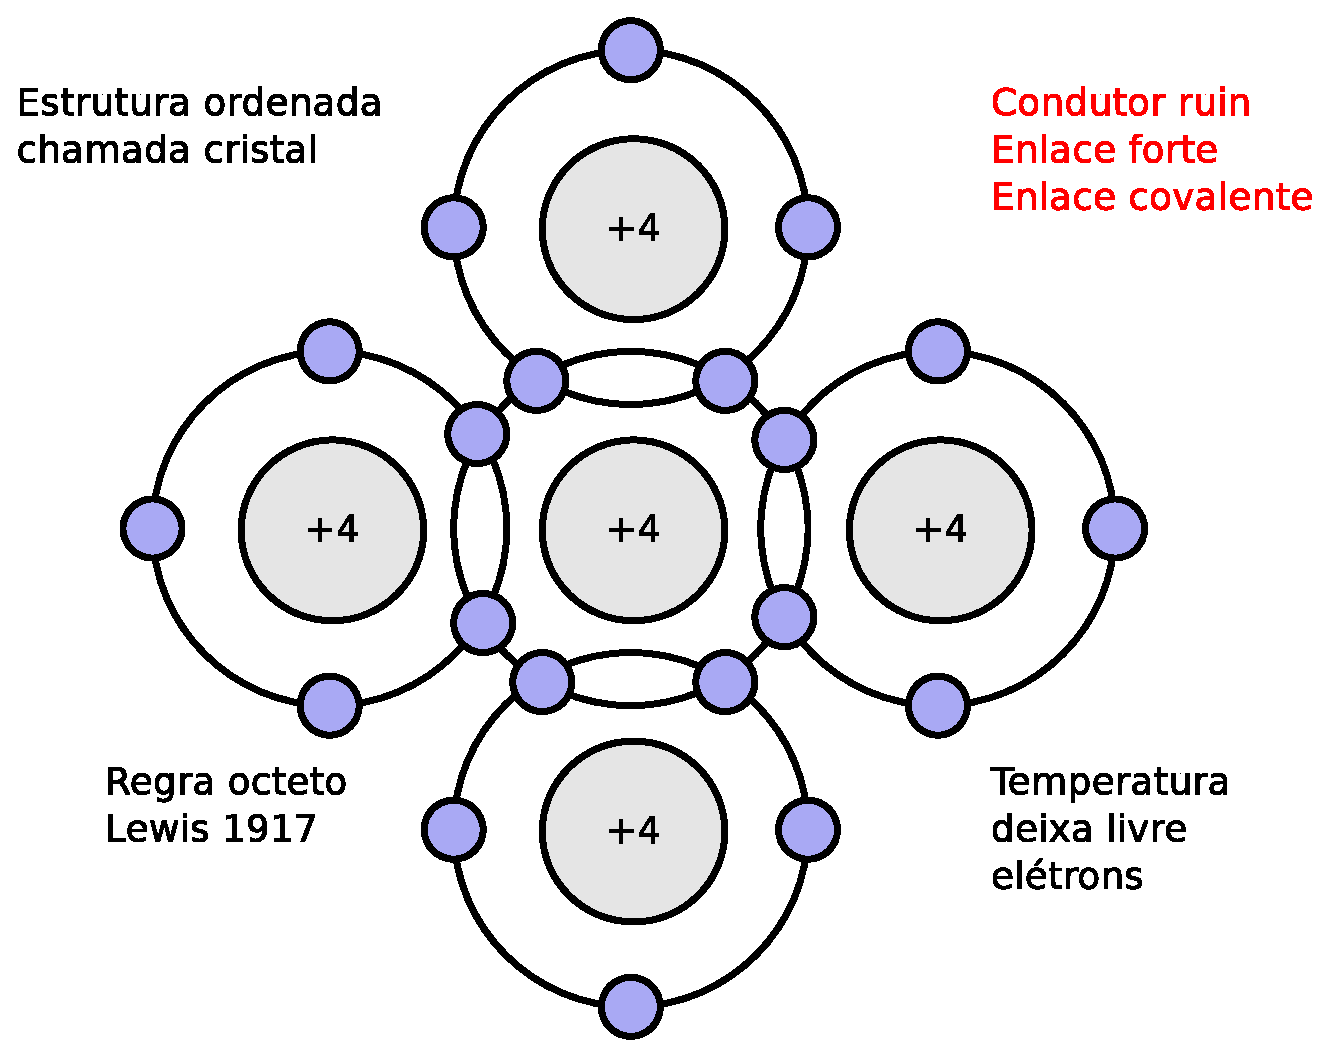
\includegraphics[width=6cm]{images/covalente.eps}
\caption{Semicondutor intrínseco (Semicondutor Puro)}
\label{fig:sige}
\end{figure}
\end{frame}

\begin{frame}{Dopagem: Semicondutor extrínseco tipo P}
\begin{figure}
\centering
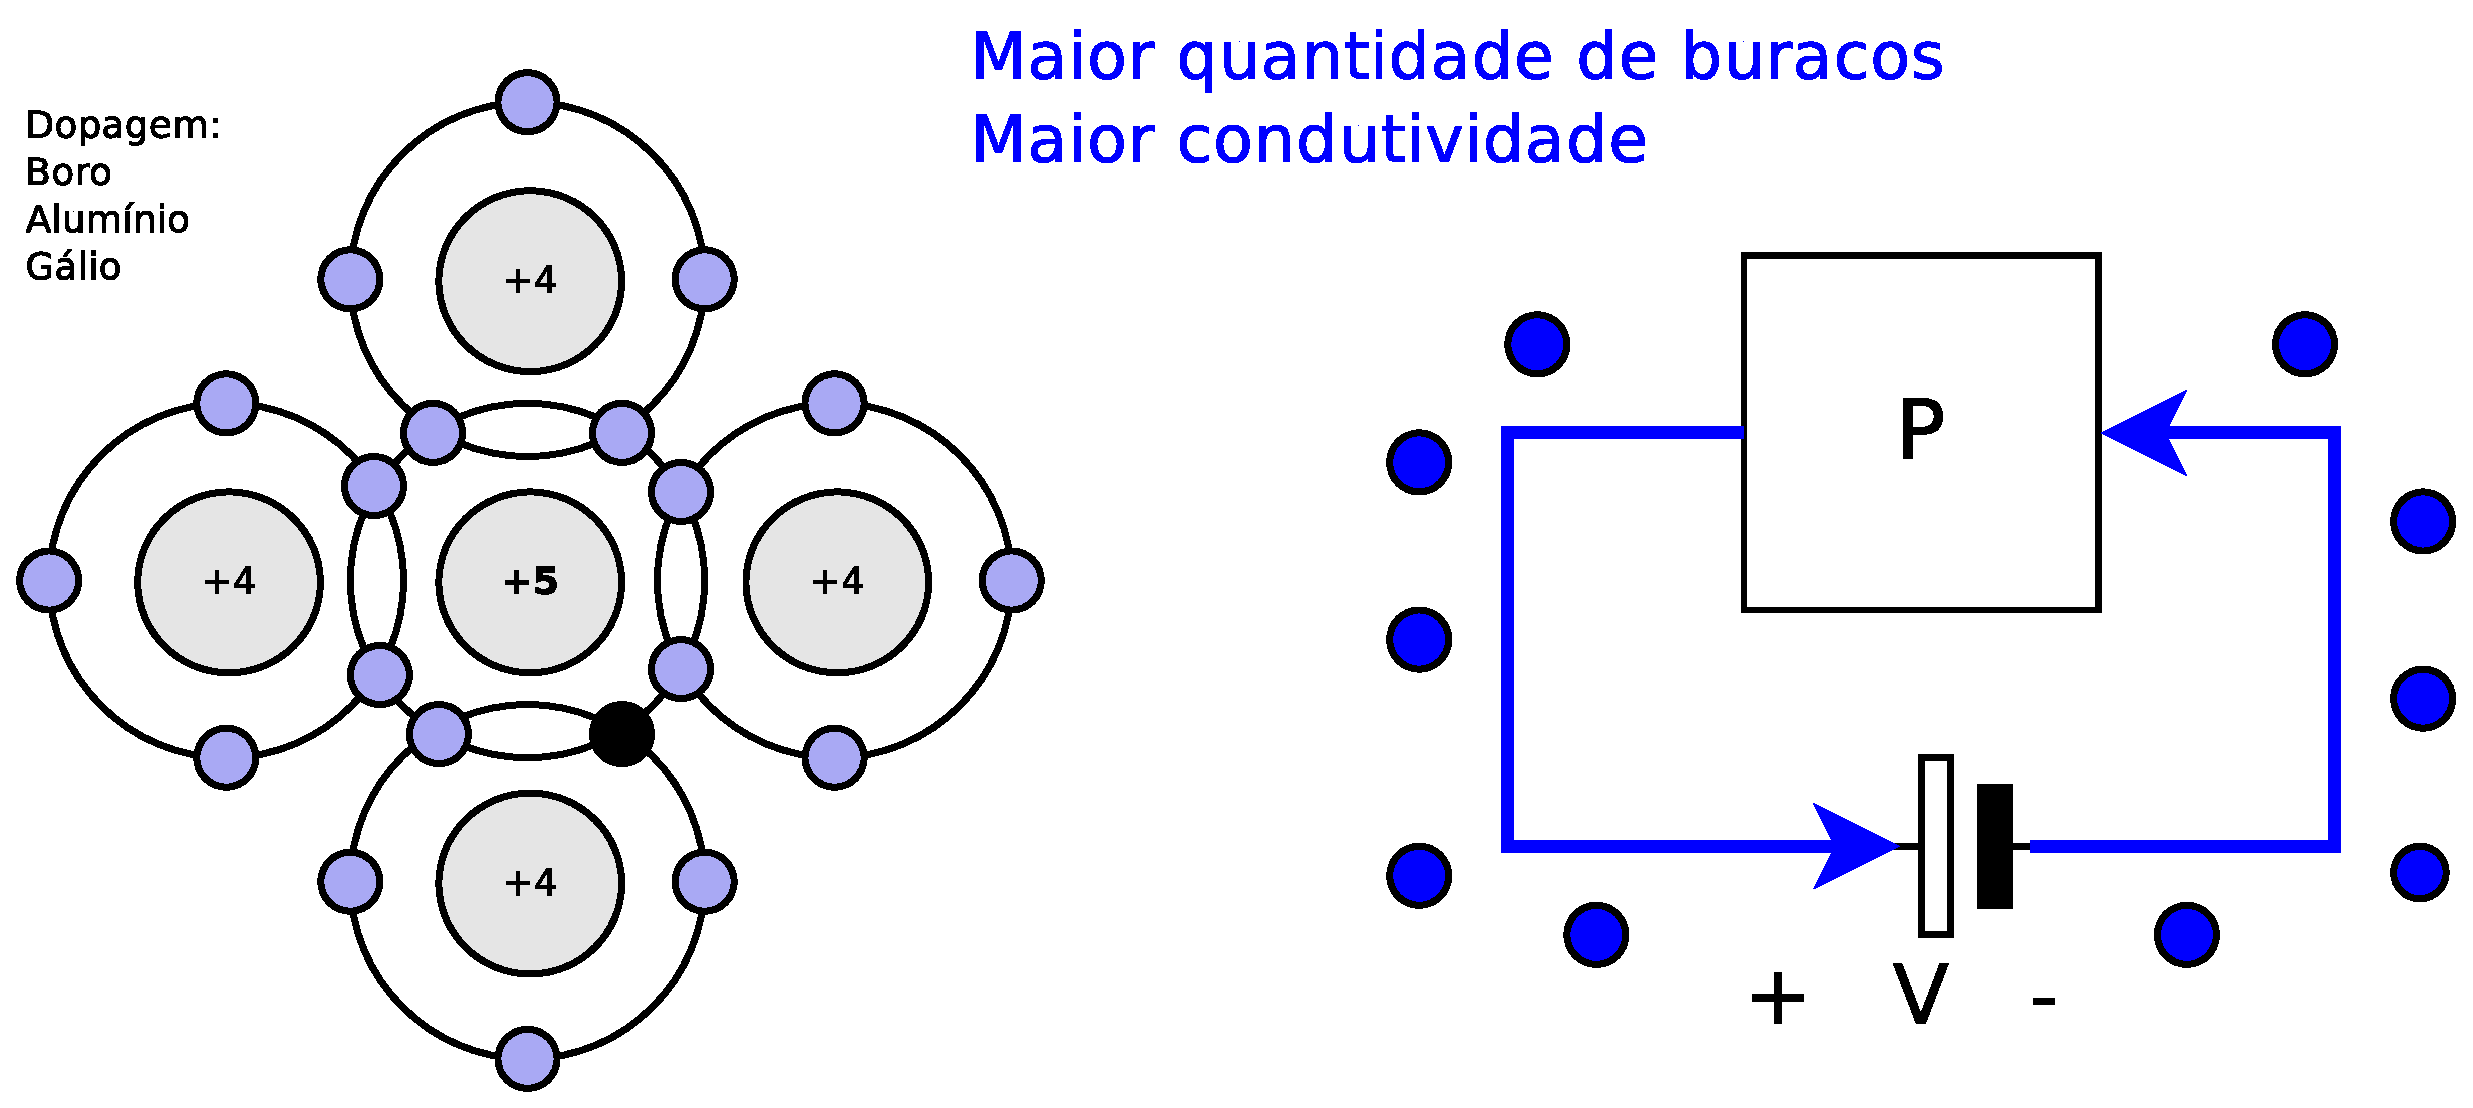
\includegraphics[width=10cm]{images/extrinsecop.eps}
\caption{Semicondutor extrínseco tipo P}
\label{fig:semip}
\end{figure}
\end{frame}

\begin{frame}{Dopagem:Semicondutor extrínseco tipo N}
\begin{figure}
\centering
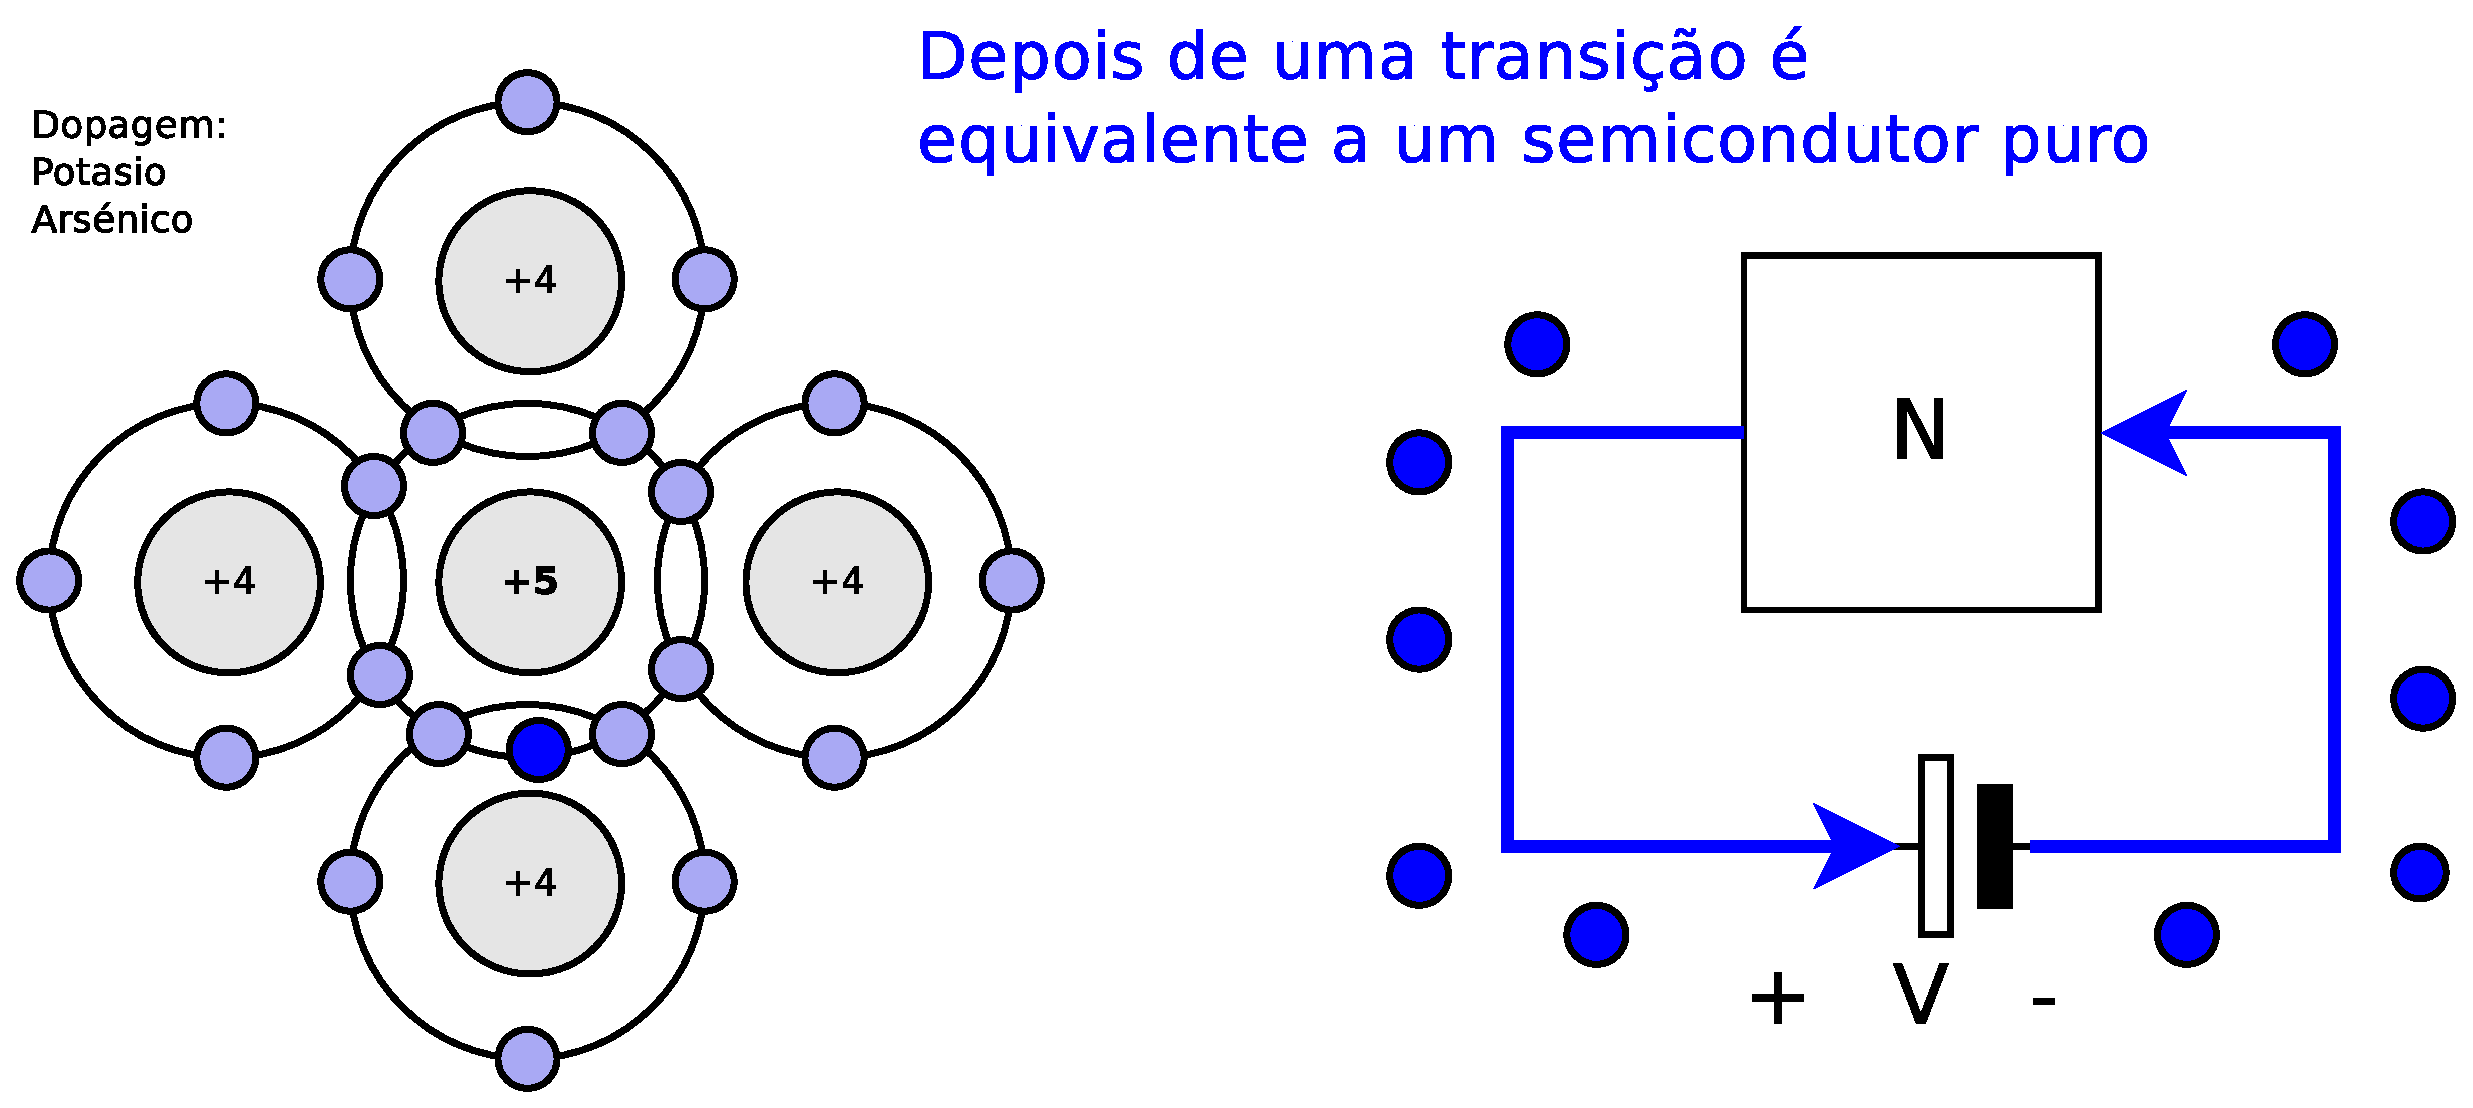
\includegraphics[width=10cm]{images/extrinsecon.eps}
\caption{Semicondutor extrínseco tipo N}
\label{fig:semin}
\end{figure}
\end{frame}

\begin{frame}{União PN  }
\begin{figure}
\centering
\includegraphics[width=9cm]{images/semipn0.eps}
\caption{União PN  }
\label{fig:semipn0}
\end{figure}
\end{frame}

\begin{frame}{União PN - Polarização direta }
\begin{figure}
\centering
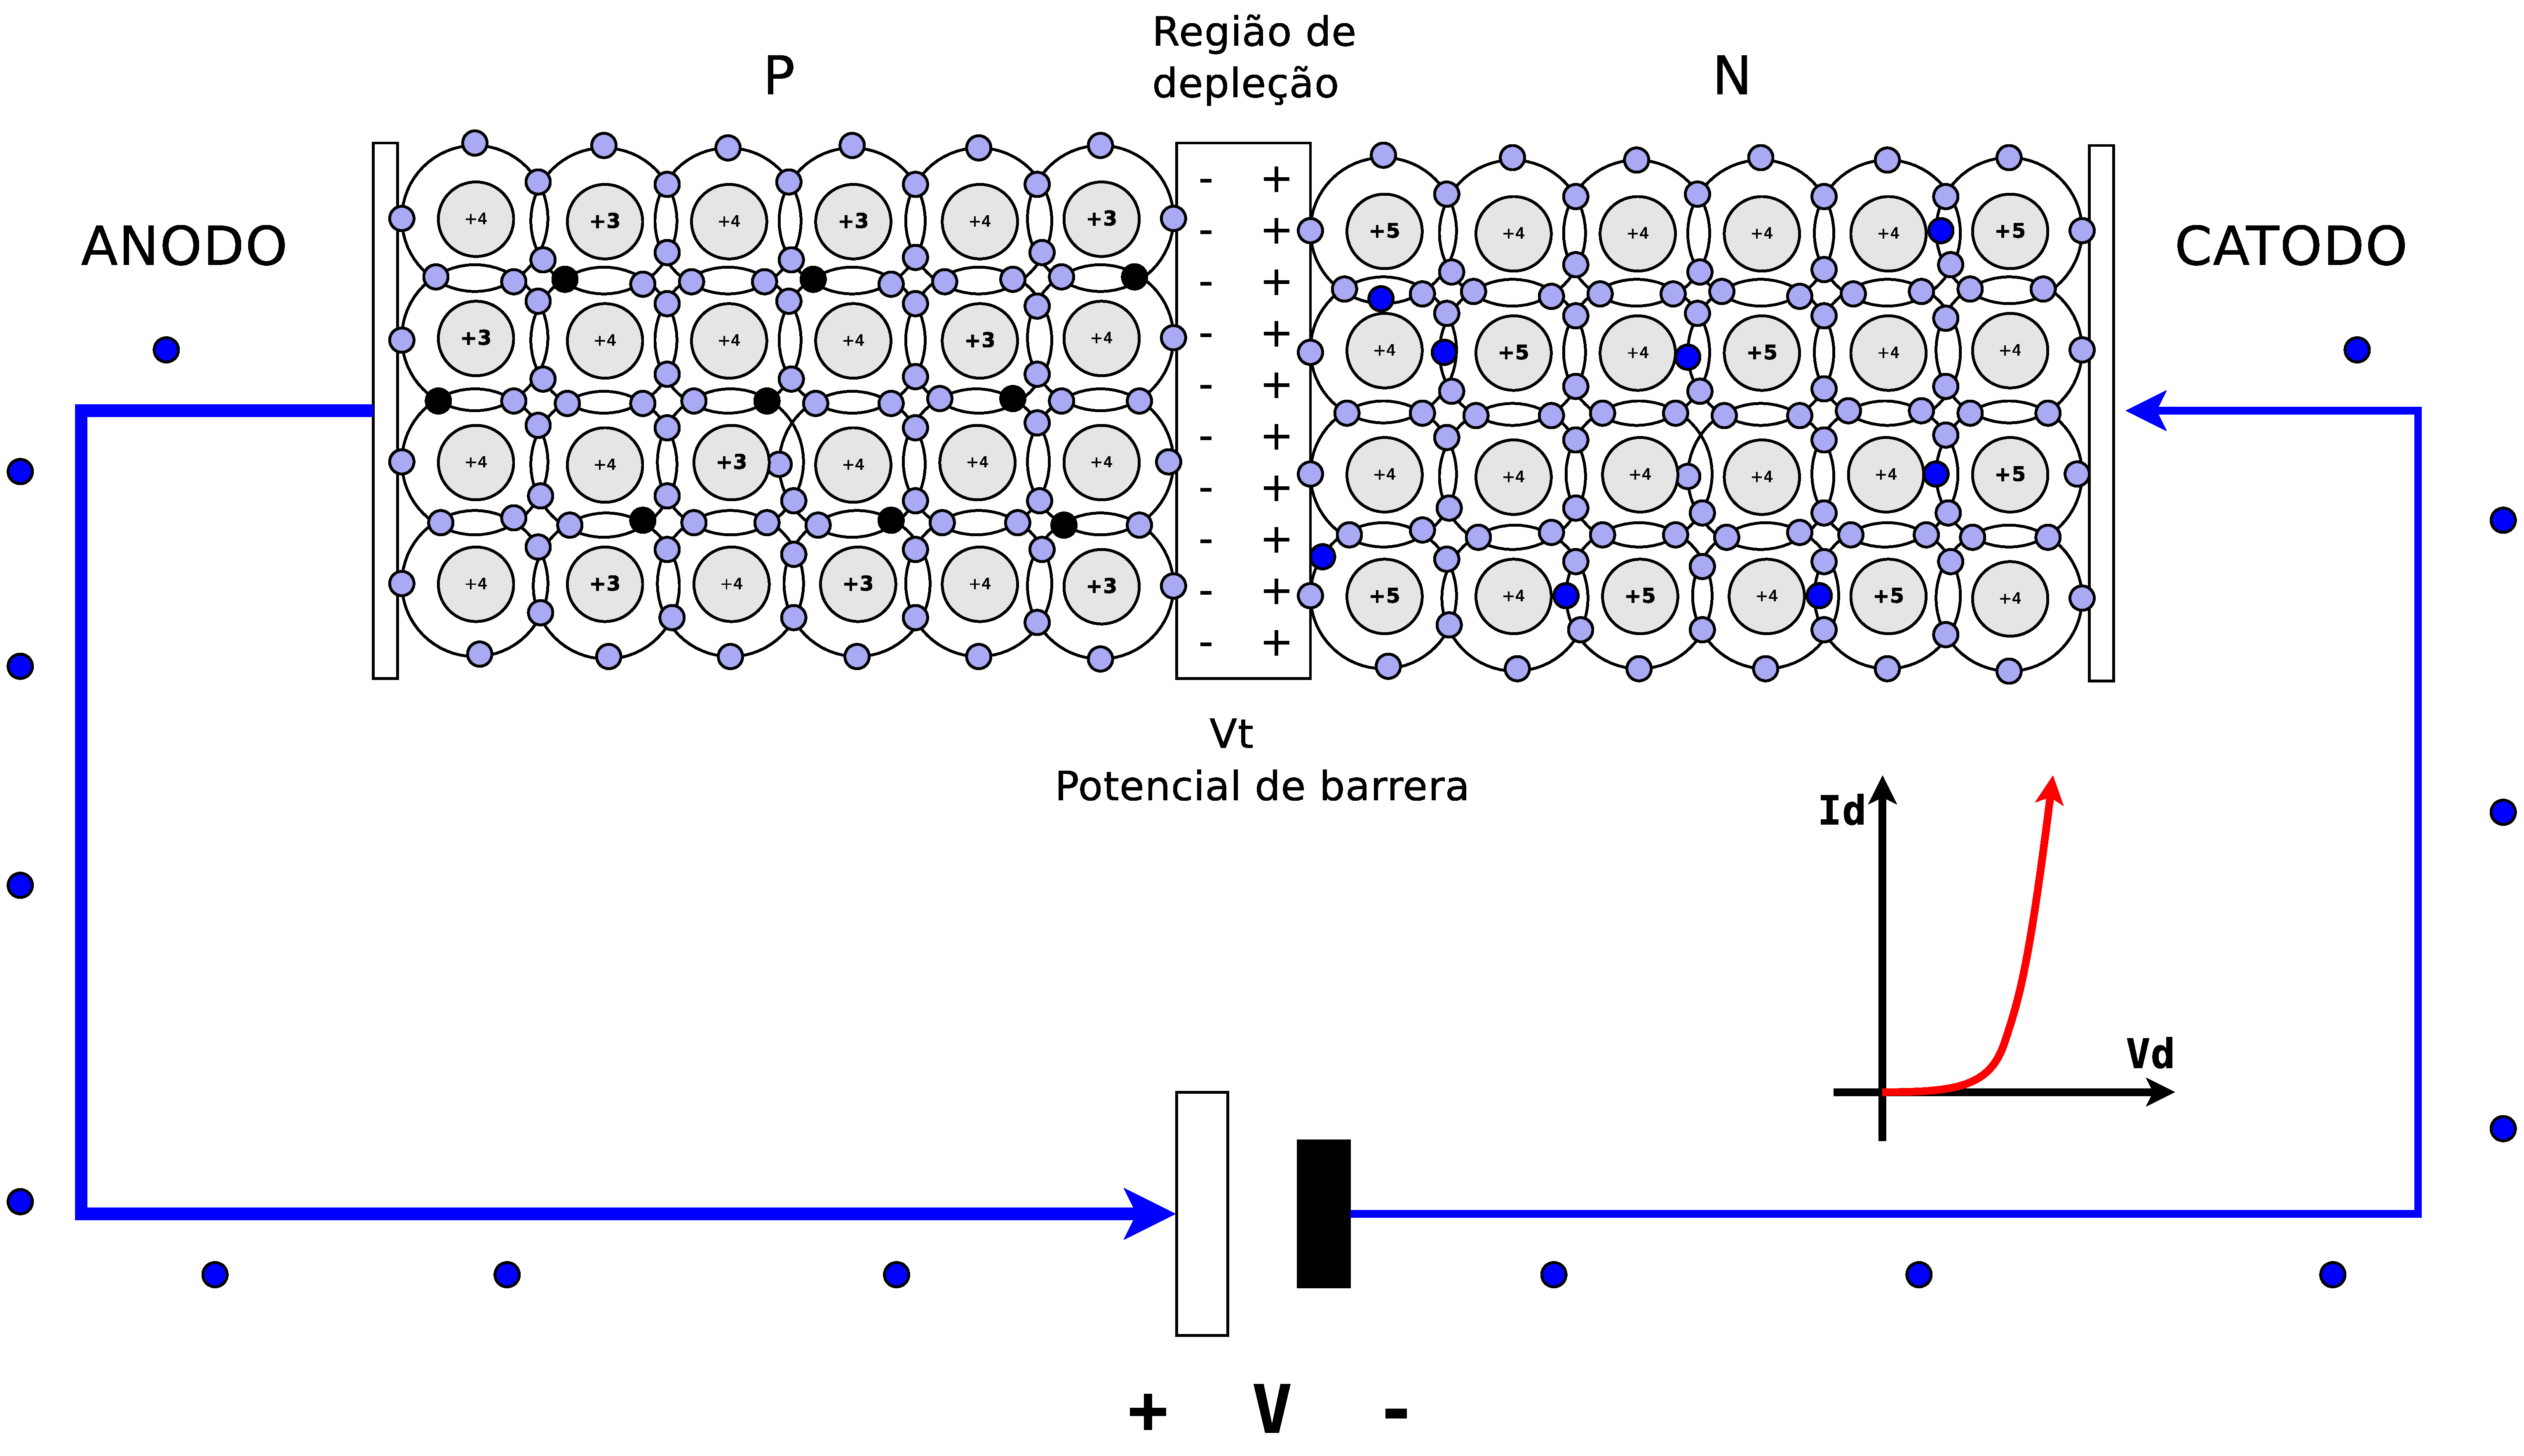
\includegraphics[width=9cm]{images/semipn.eps}
\caption{Polarização direta}
\label{fig:semipn0}
\end{figure}
\end{frame}

\begin{frame}{União PN - Polarização inversa }
\begin{figure}
\centering
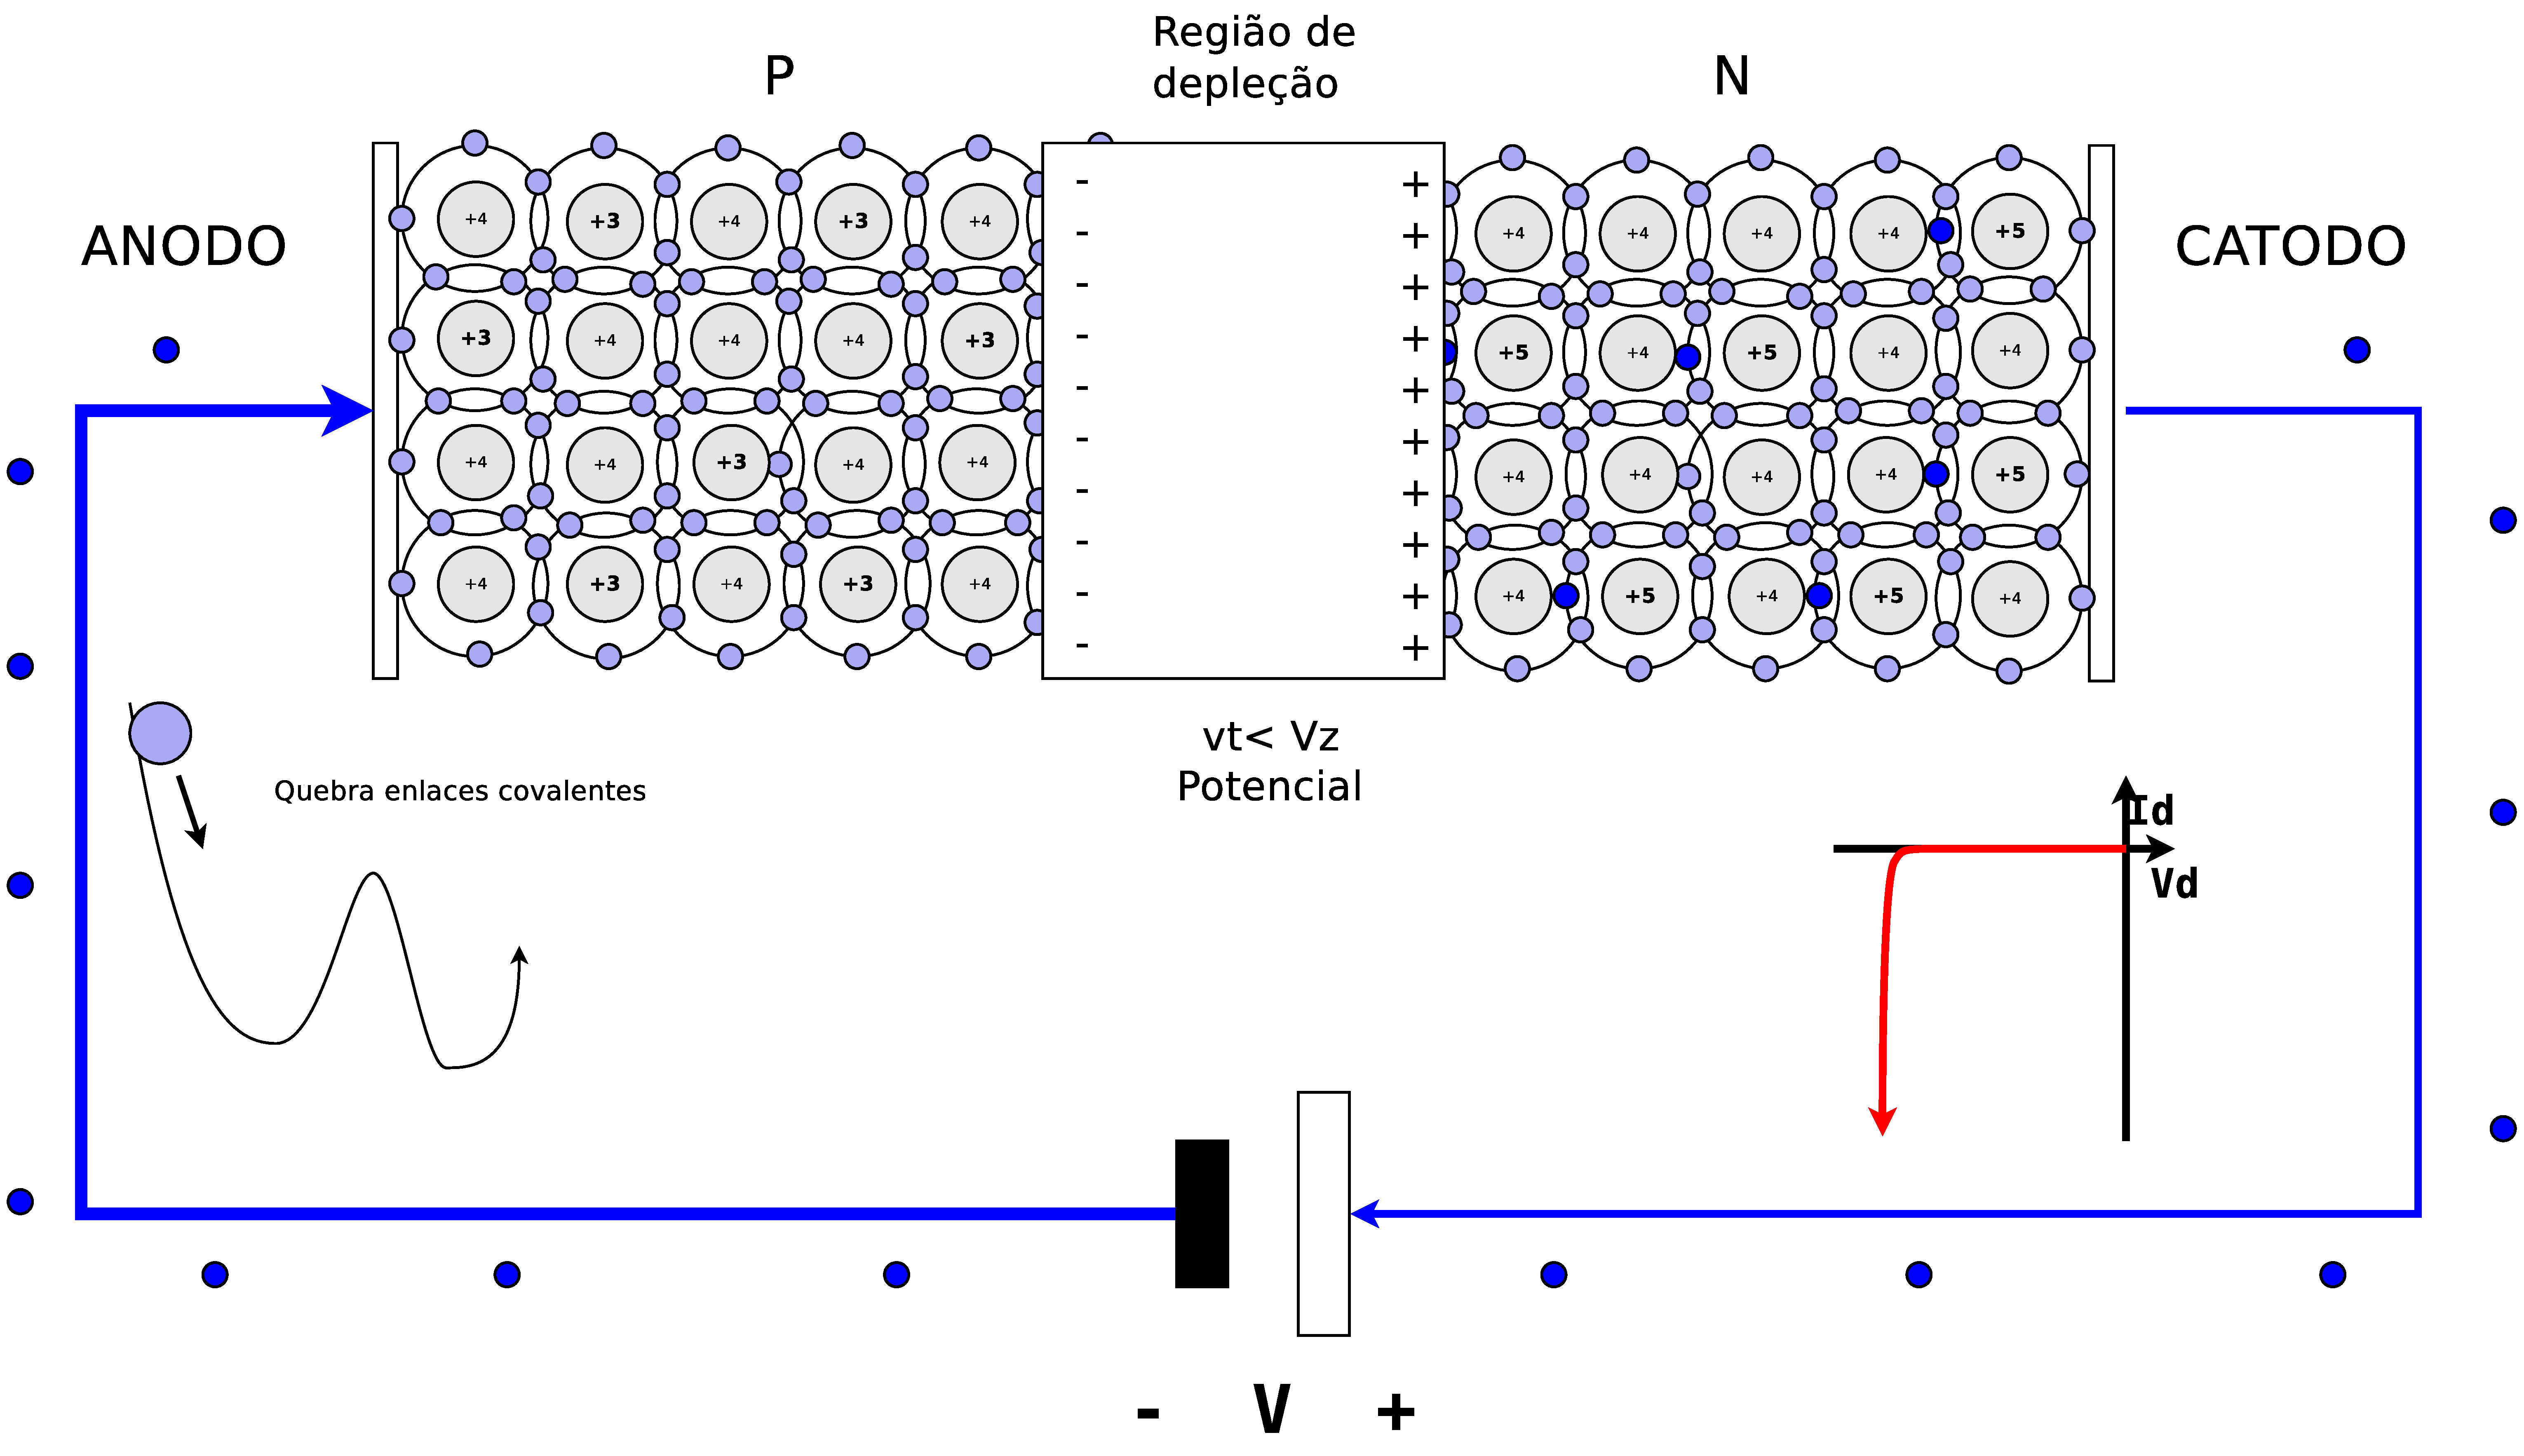
\includegraphics[width=9cm]{images/semipn2.eps}
\caption{Polarização inversa}
\label{fig:semipn0}
\end{figure}
\end{frame}

\begin{frame}{União NPN e PNP}
\begin{figure}
\centering
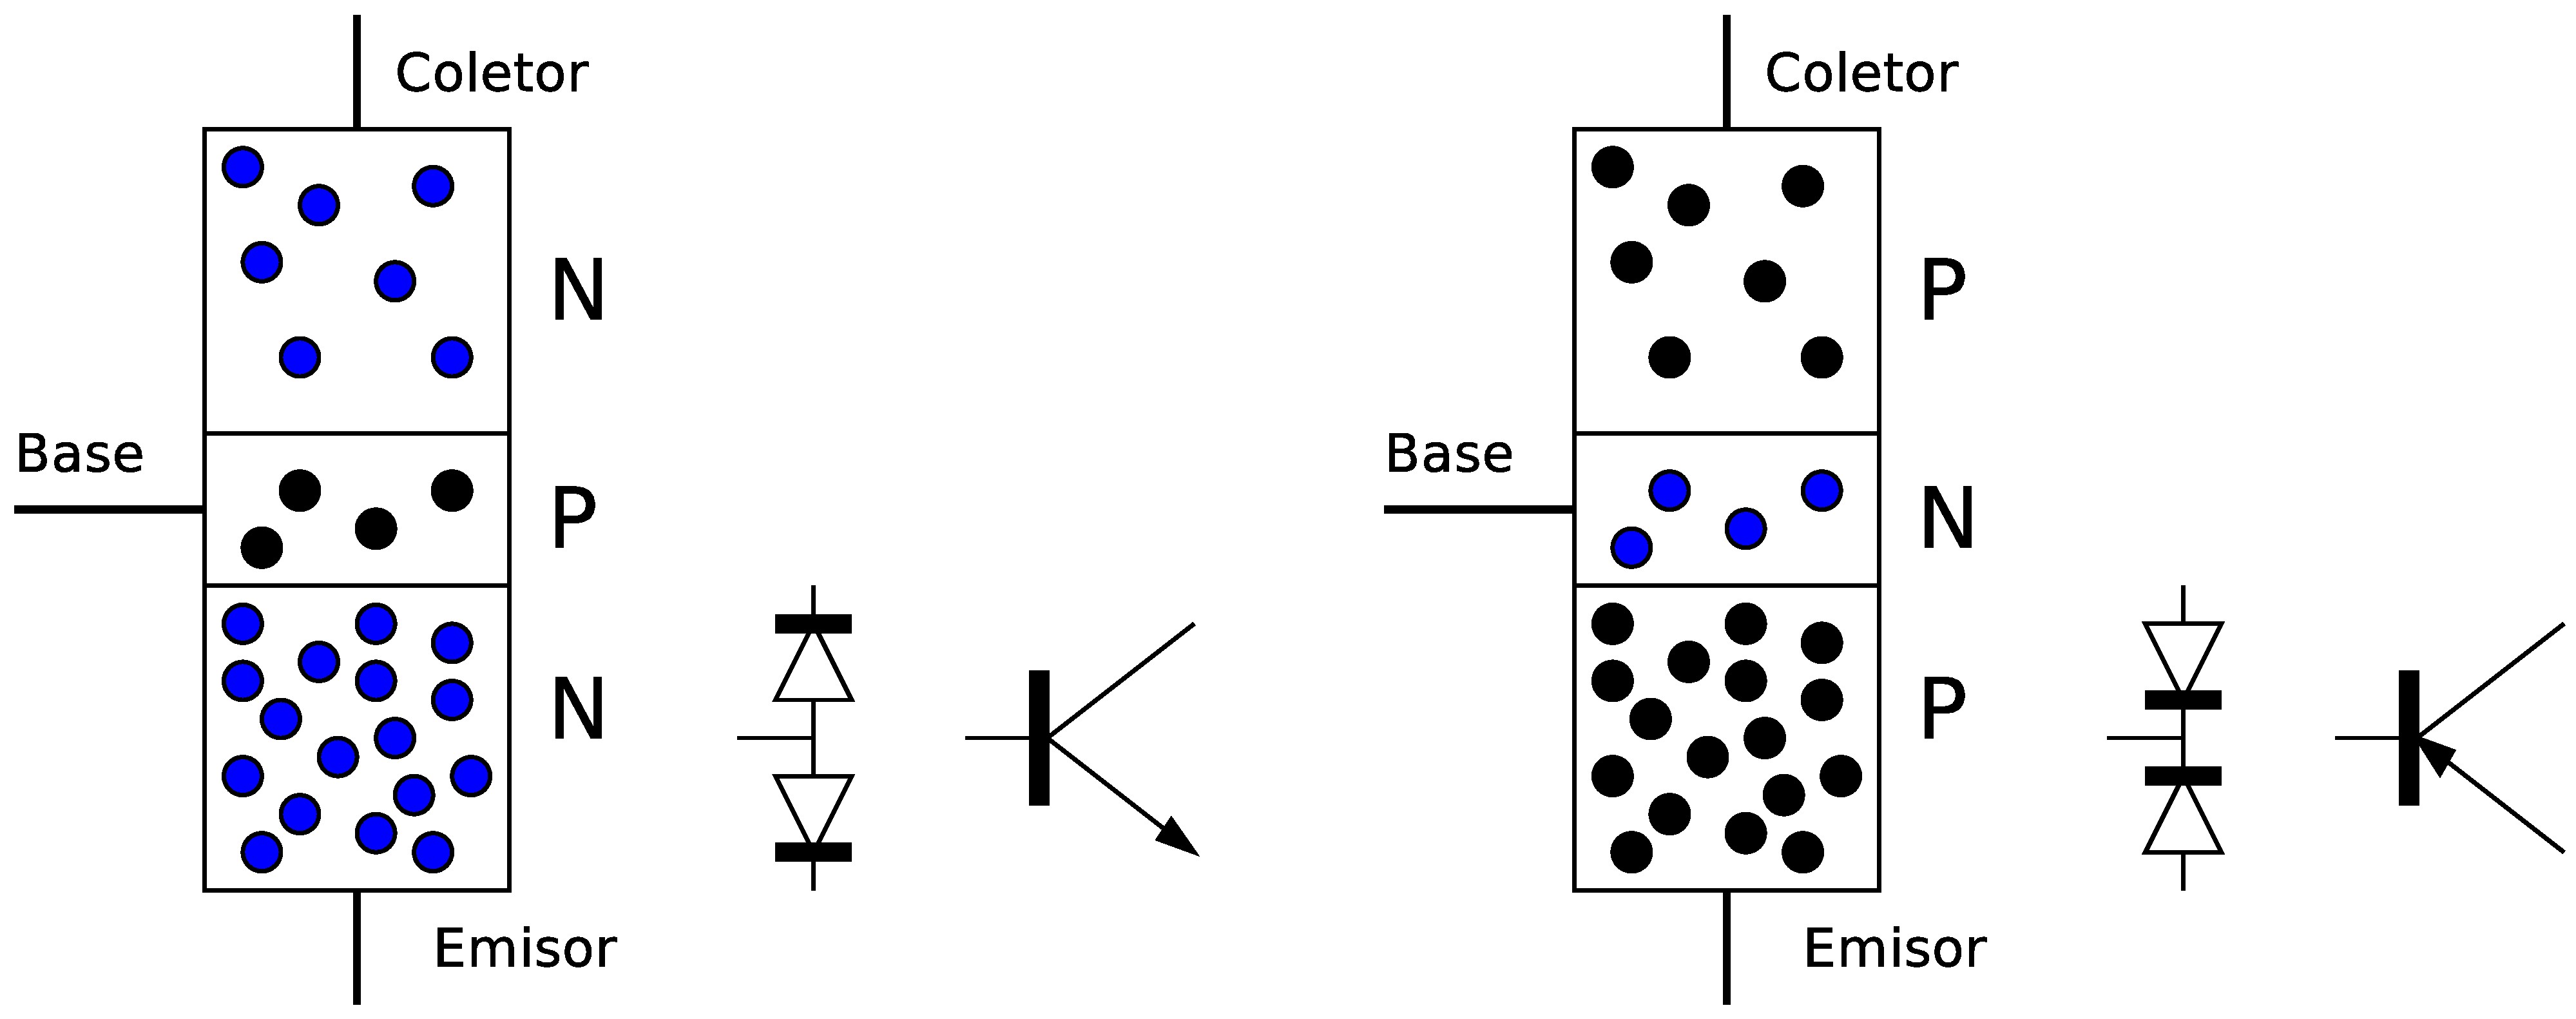
\includegraphics[width=10cm]{images/npn-pnp.eps}
\caption{Transistor BJT - Sem polarização}
\label{fig:npnpnp}
\end{figure}
\end{frame}

%https://www.youtube.com/watch?v=l_EG544soDg

\begin{frame}{Transistor NPN polarizado }
\begin{figure}
\centering
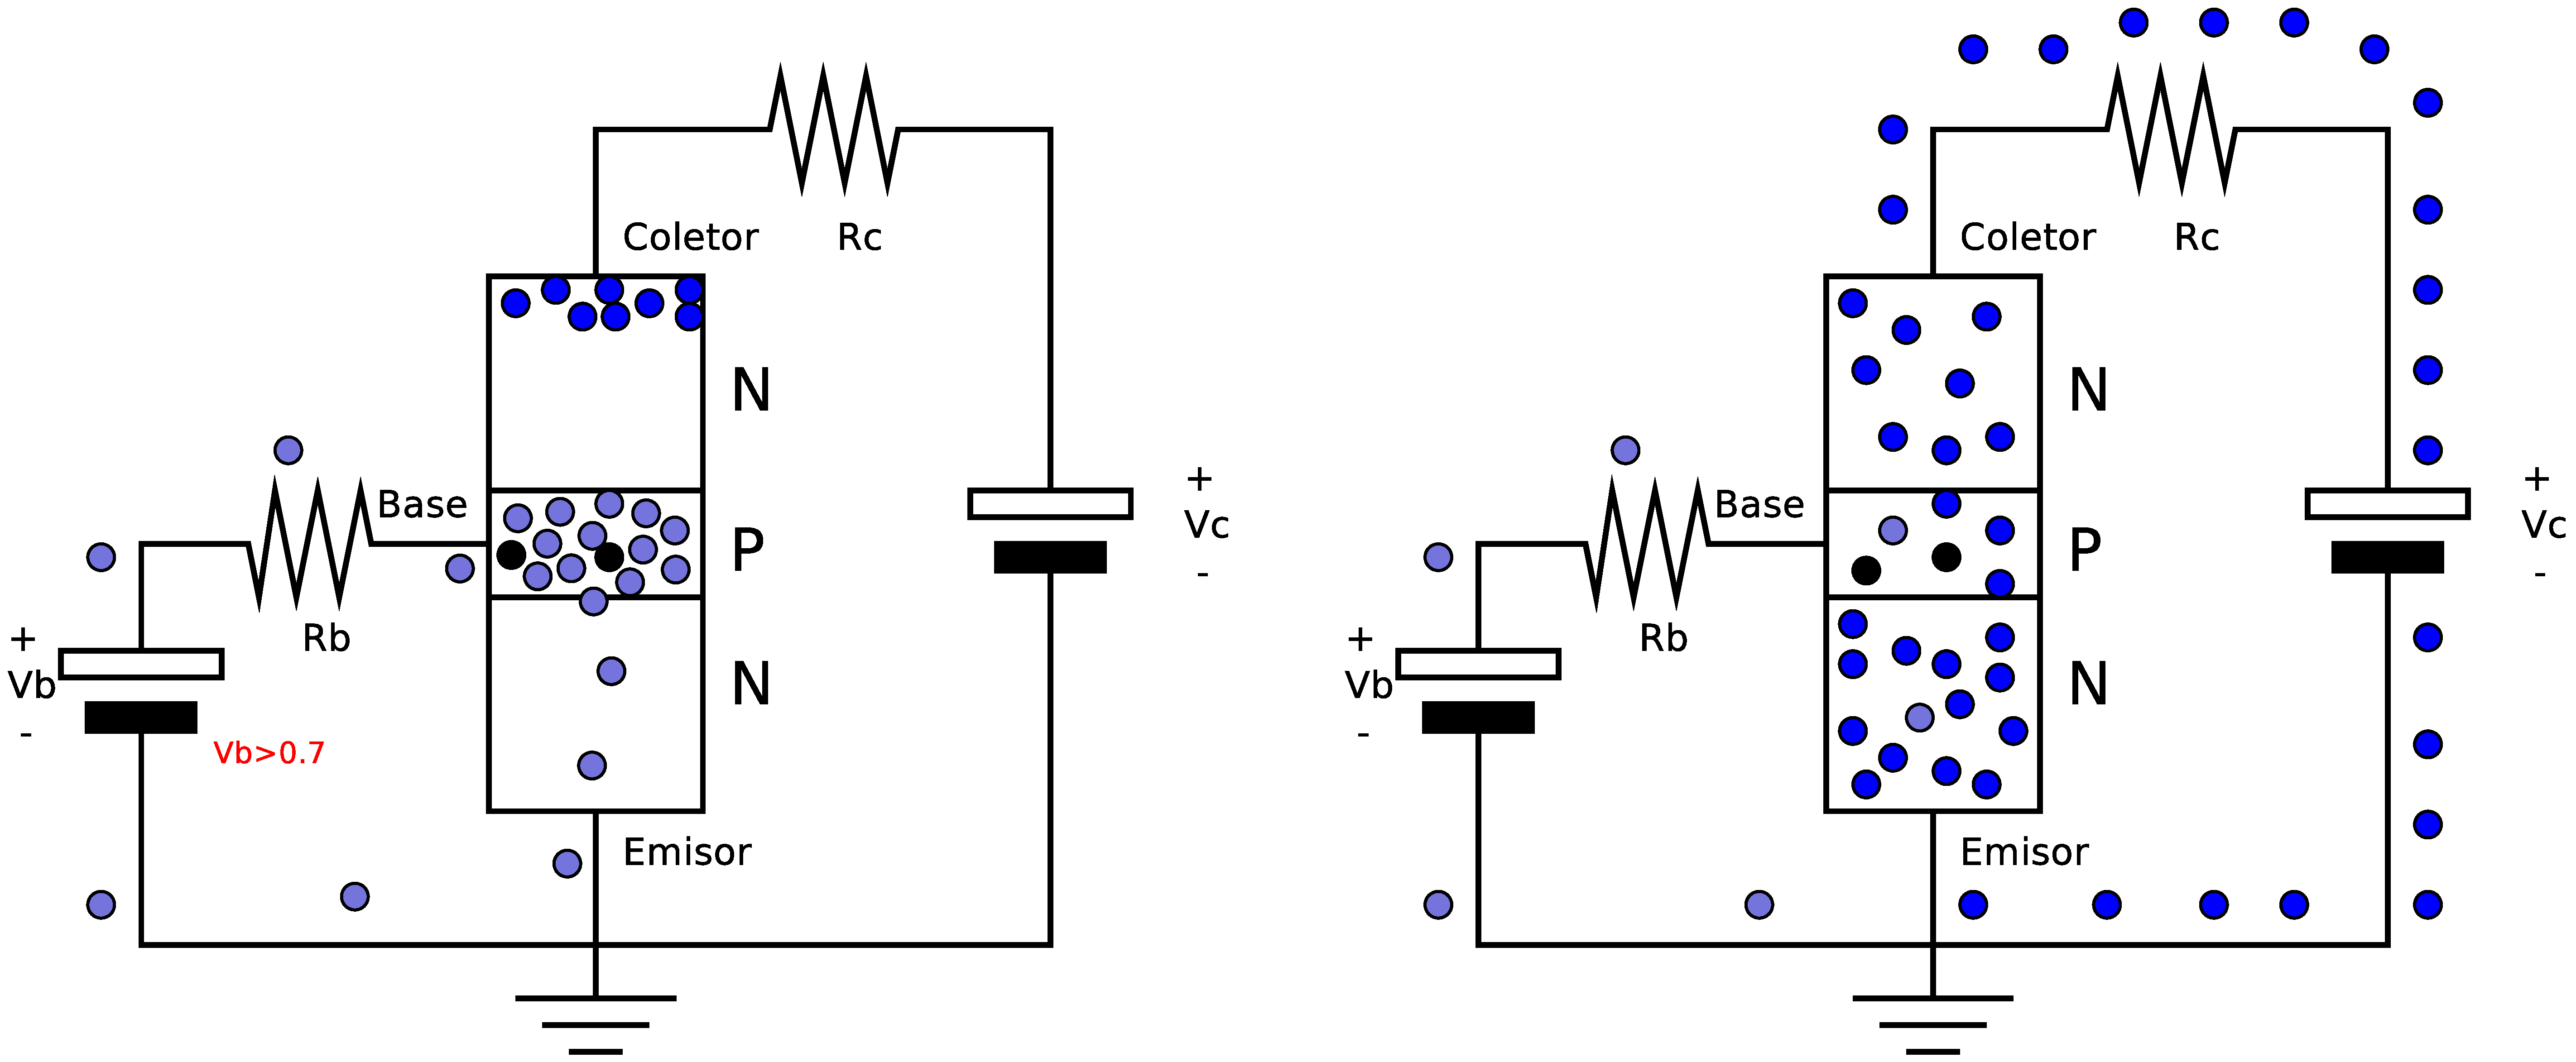
\includegraphics[width=10cm]{images/npn.eps}
\caption{Transistor BJT}
\label{fig:npn}
\end{figure}
\end{frame}

%%%%%%%%%%%%%%%%%%%%%%%%%%%%%%%%%%%%%%%%%%%%%%%%%%%%%%%%%%%%%%%%%%%%%%%%%%%%%%%%
%%%%%%%%%%%%%%%%%%%%%%%%%%%%%%%%%%%%%%%%%%%%%%%%%%%%%%%%%%%%%%%%%%%%%%%%%%%%%%%%
%%%%%%%%%%%%%%%%%%%%%%%%%%%%%%%%%%%%%%%%%%%%%%%%%%%%%%%%%%%%%%%%%%%%%%%%%%%%%%%%
\section{Caraterísticas}



\begin{frame}{Ganho de corrente num BJT em DC  }
\begin{figure}
\centering
\includegraphics[width=10cm]{images/ganancia.eps}
\caption{NPN - Ganho de corrente}
\label{fig:ganancia}
\end{figure}
\end{frame}

\begin{frame}{Ganho de corrente num BJT em DC  }
\begin{figure}
\centering
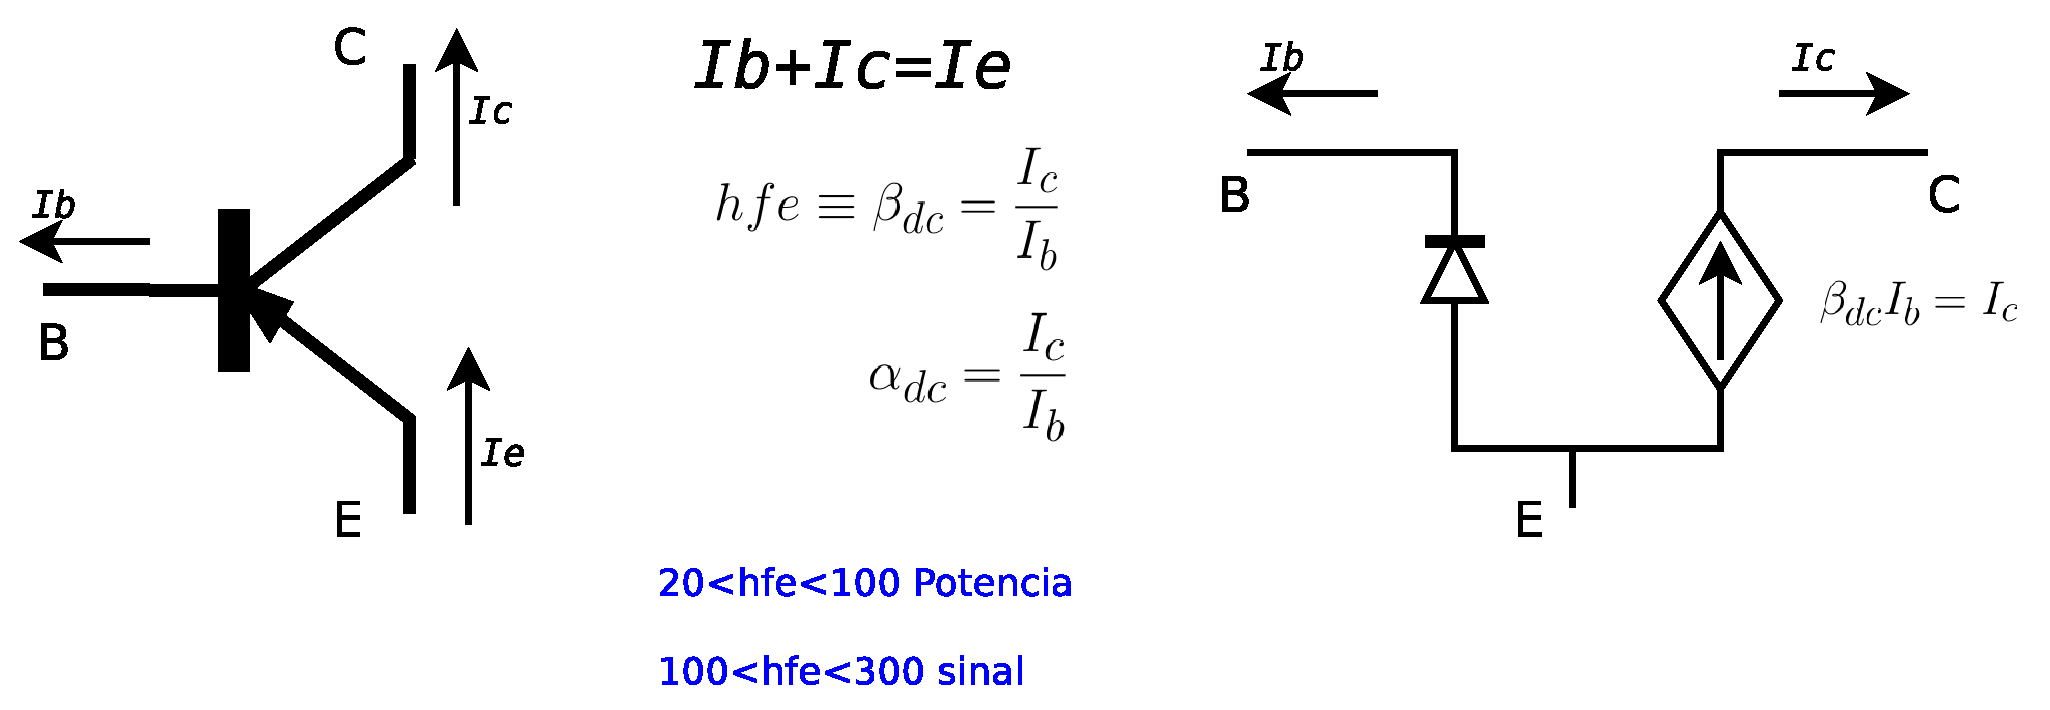
\includegraphics[width=10cm]{images/ganancia2.eps}
\caption{PNP - Ganho de corrente}
\label{fig:ganancia2}
\end{figure}
\end{frame}

\begin{frame}{Curva do transistor}
\begin{figure}
\centering
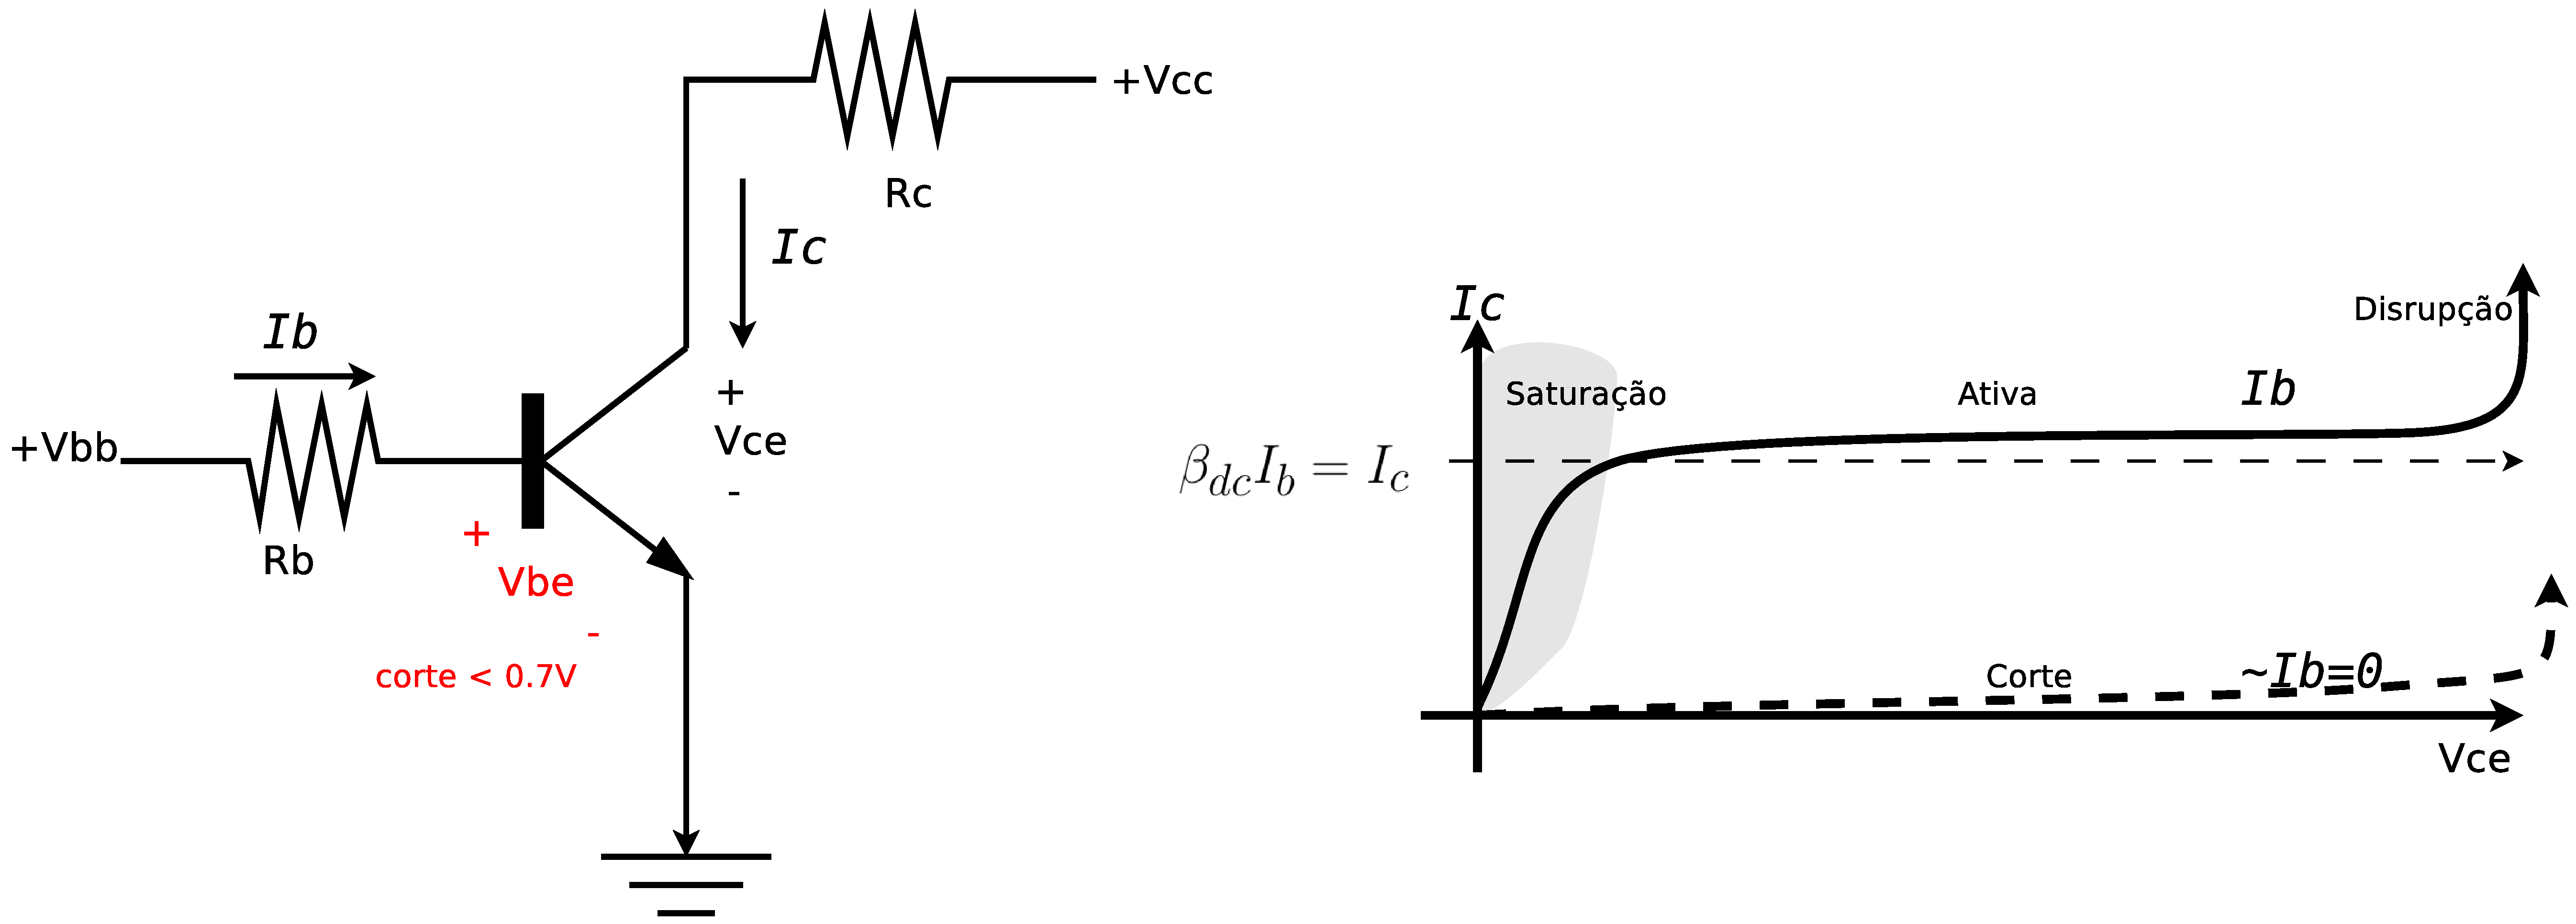
\includegraphics[width=10cm]{images/emisorcomun.eps}
\caption{Curva característica do transistor}
\label{fig:emisorcomun}
\end{figure}
\end{frame}

\begin{frame}{Corte e saturação }
\begin{figure}
\centering
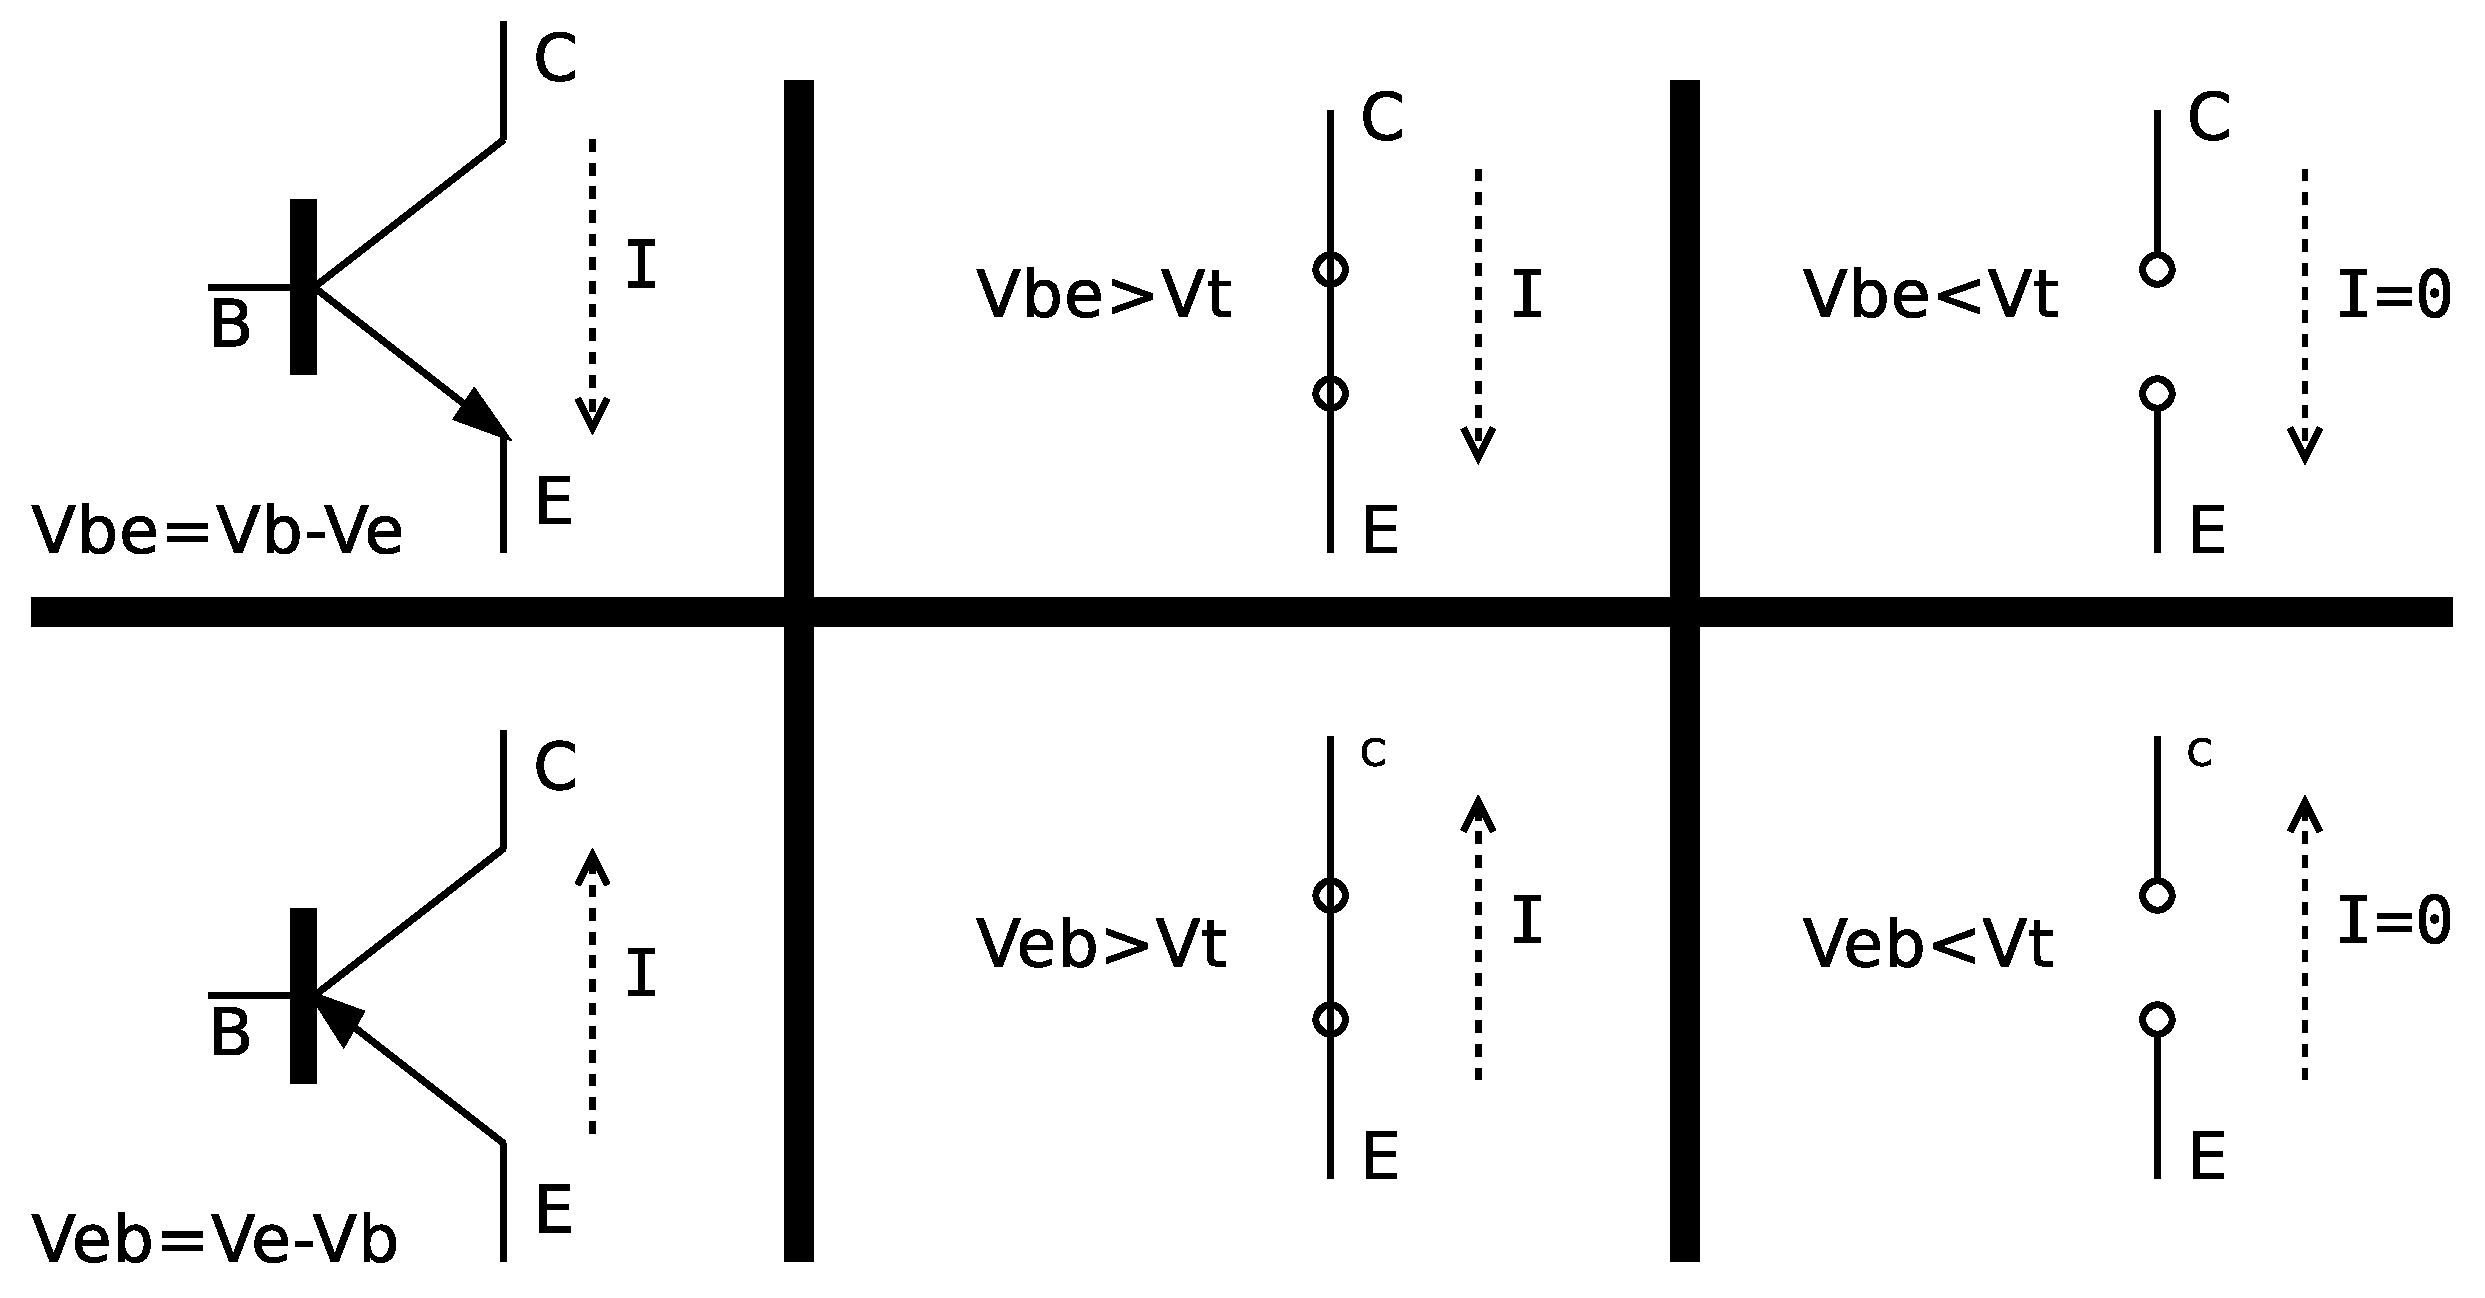
\includegraphics[width=9cm]{images/simple.eps}
\caption{Descrição  do BJT em saturação e corte}
\label{fig:simples2}
\end{figure}
\end{frame}

\begin{frame}{Levar um transistor na região de corte}
\begin{figure}
\centering
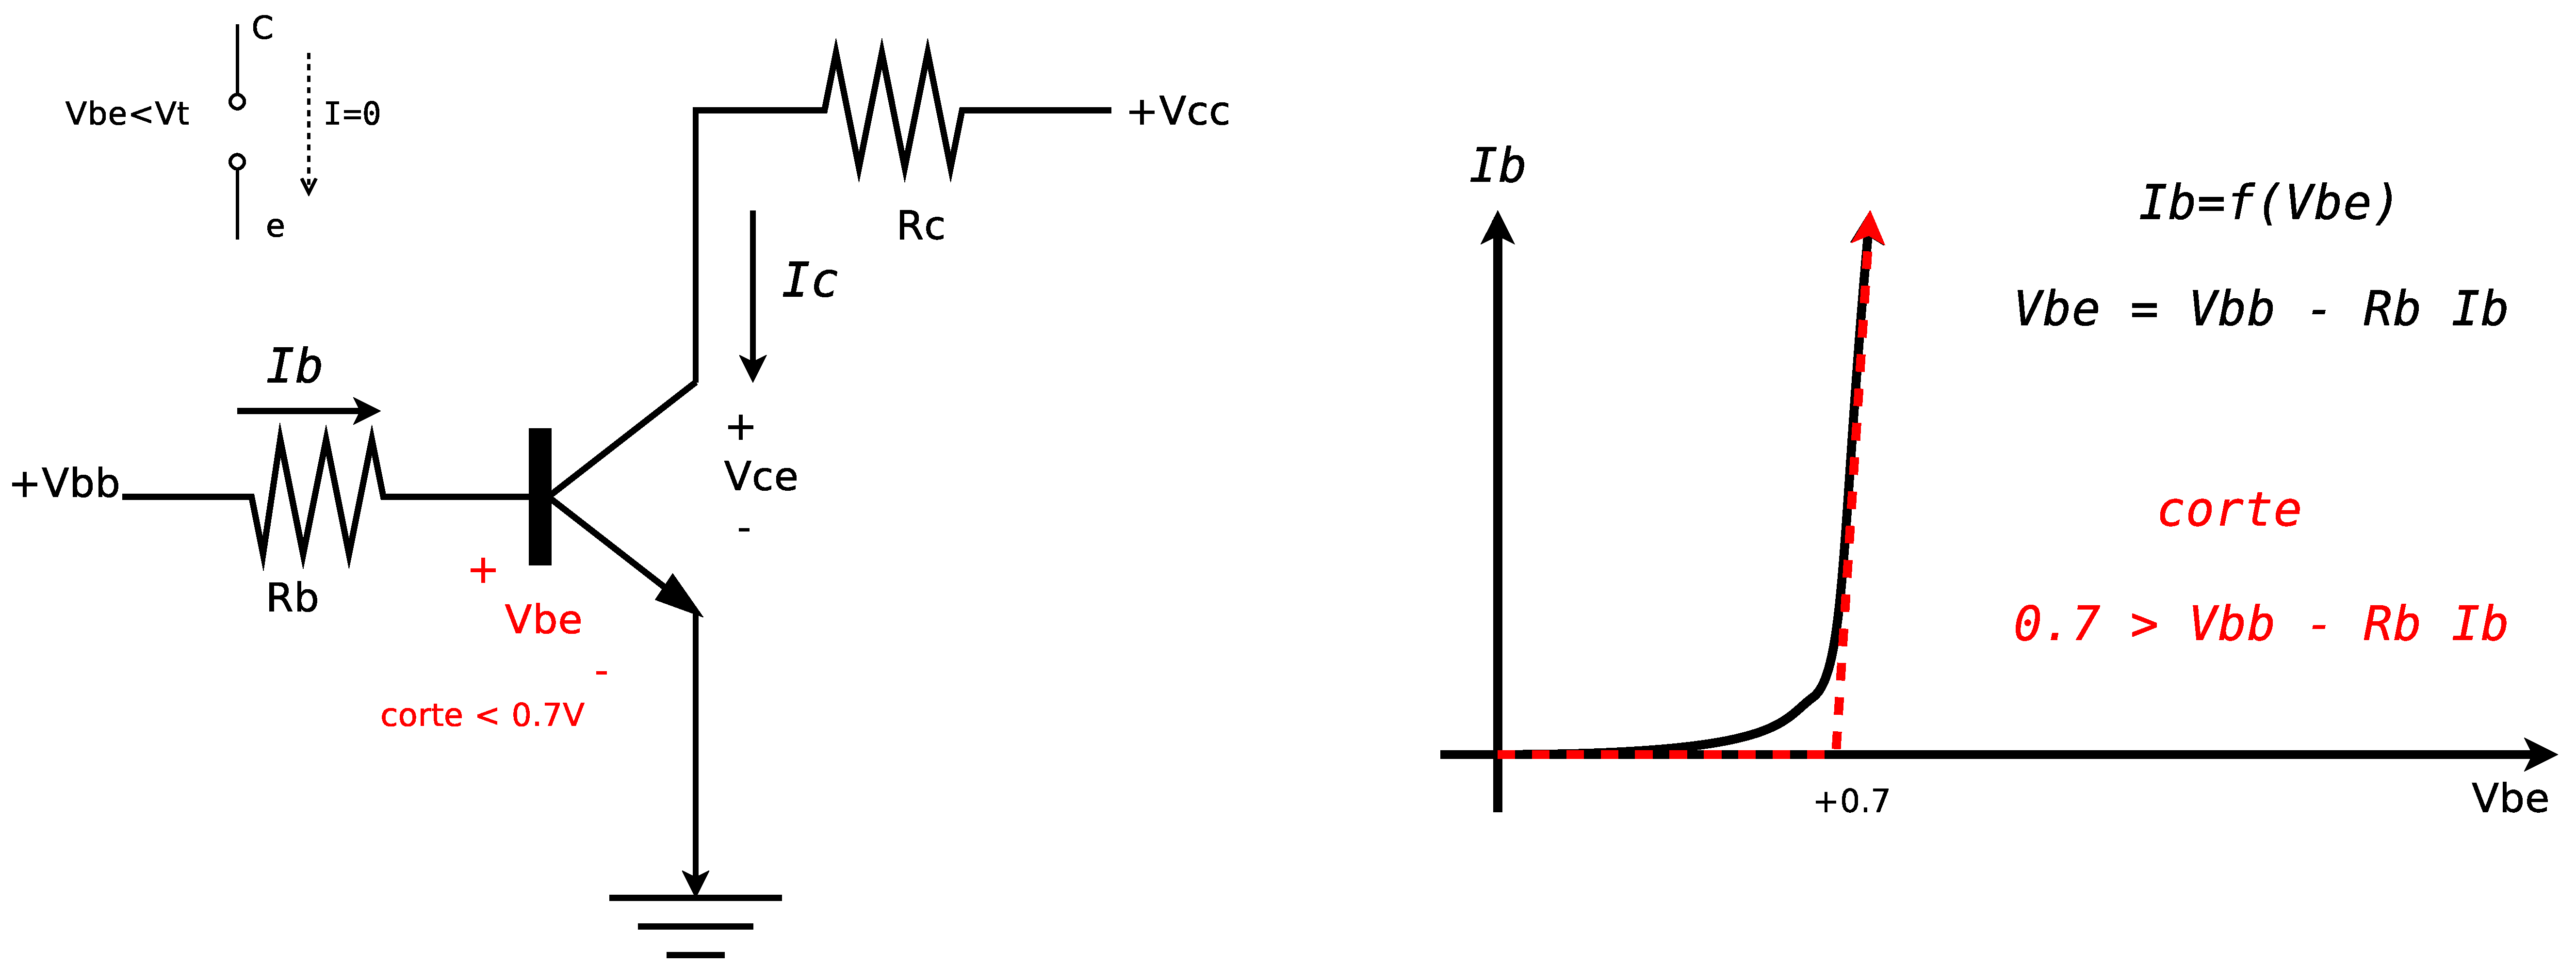
\includegraphics[width=10cm]{images/emisorcomun1.eps}
\caption{Transistor em corte}
\label{fig:emisorcomun1}
\end{figure}
\end{frame}

\begin{frame}{Levar um transistor na região de ativa}
\begin{figure}
\centering
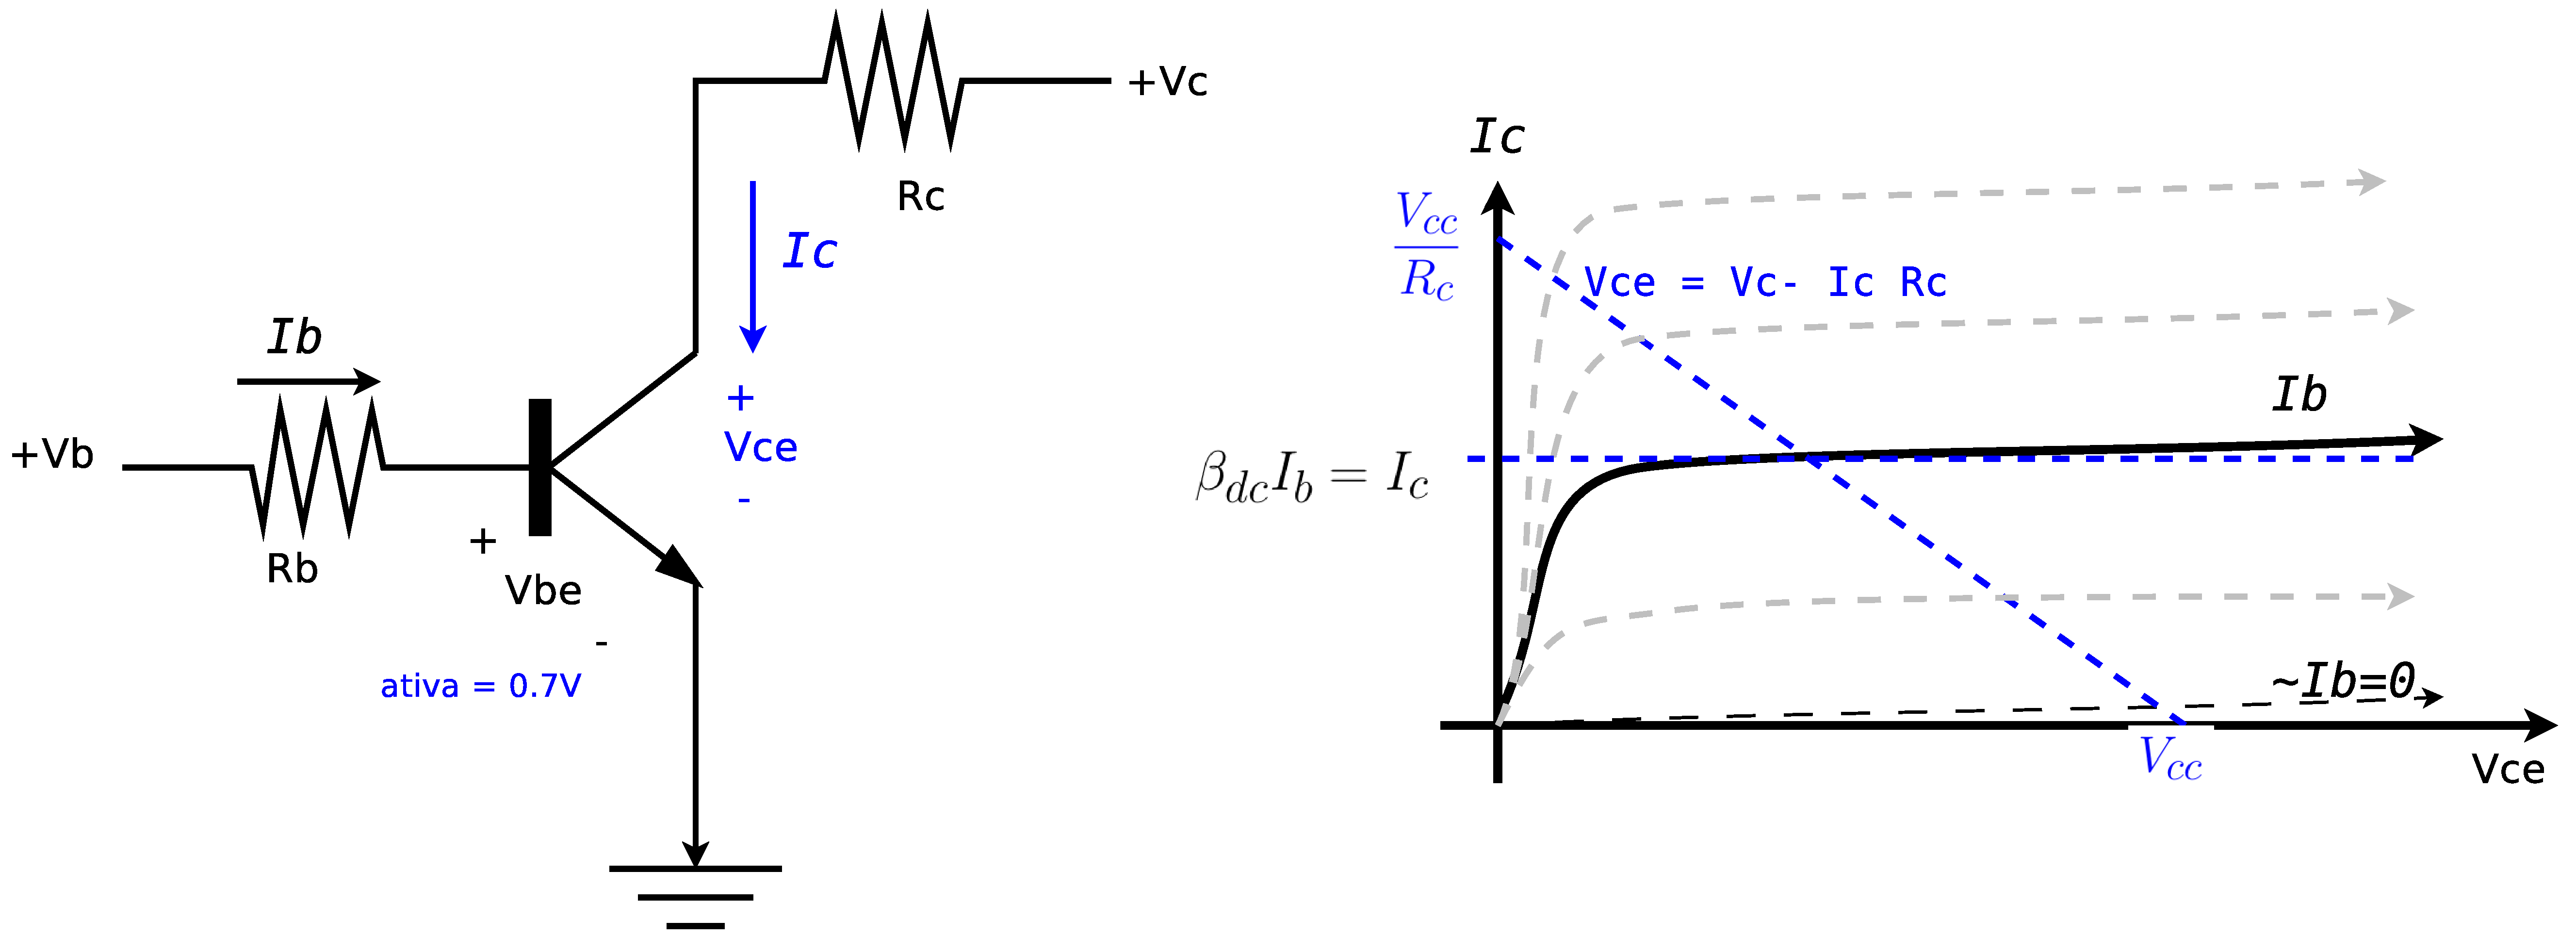
\includegraphics[width=10cm]{images/emisorcomun2.eps}
\caption{Transistor na região ativa}
\label{fig:emisorcomun2}
\end{figure}
\end{frame}


\begin{frame}{Levar um transistor na região de saturação}
\begin{figure}
\centering
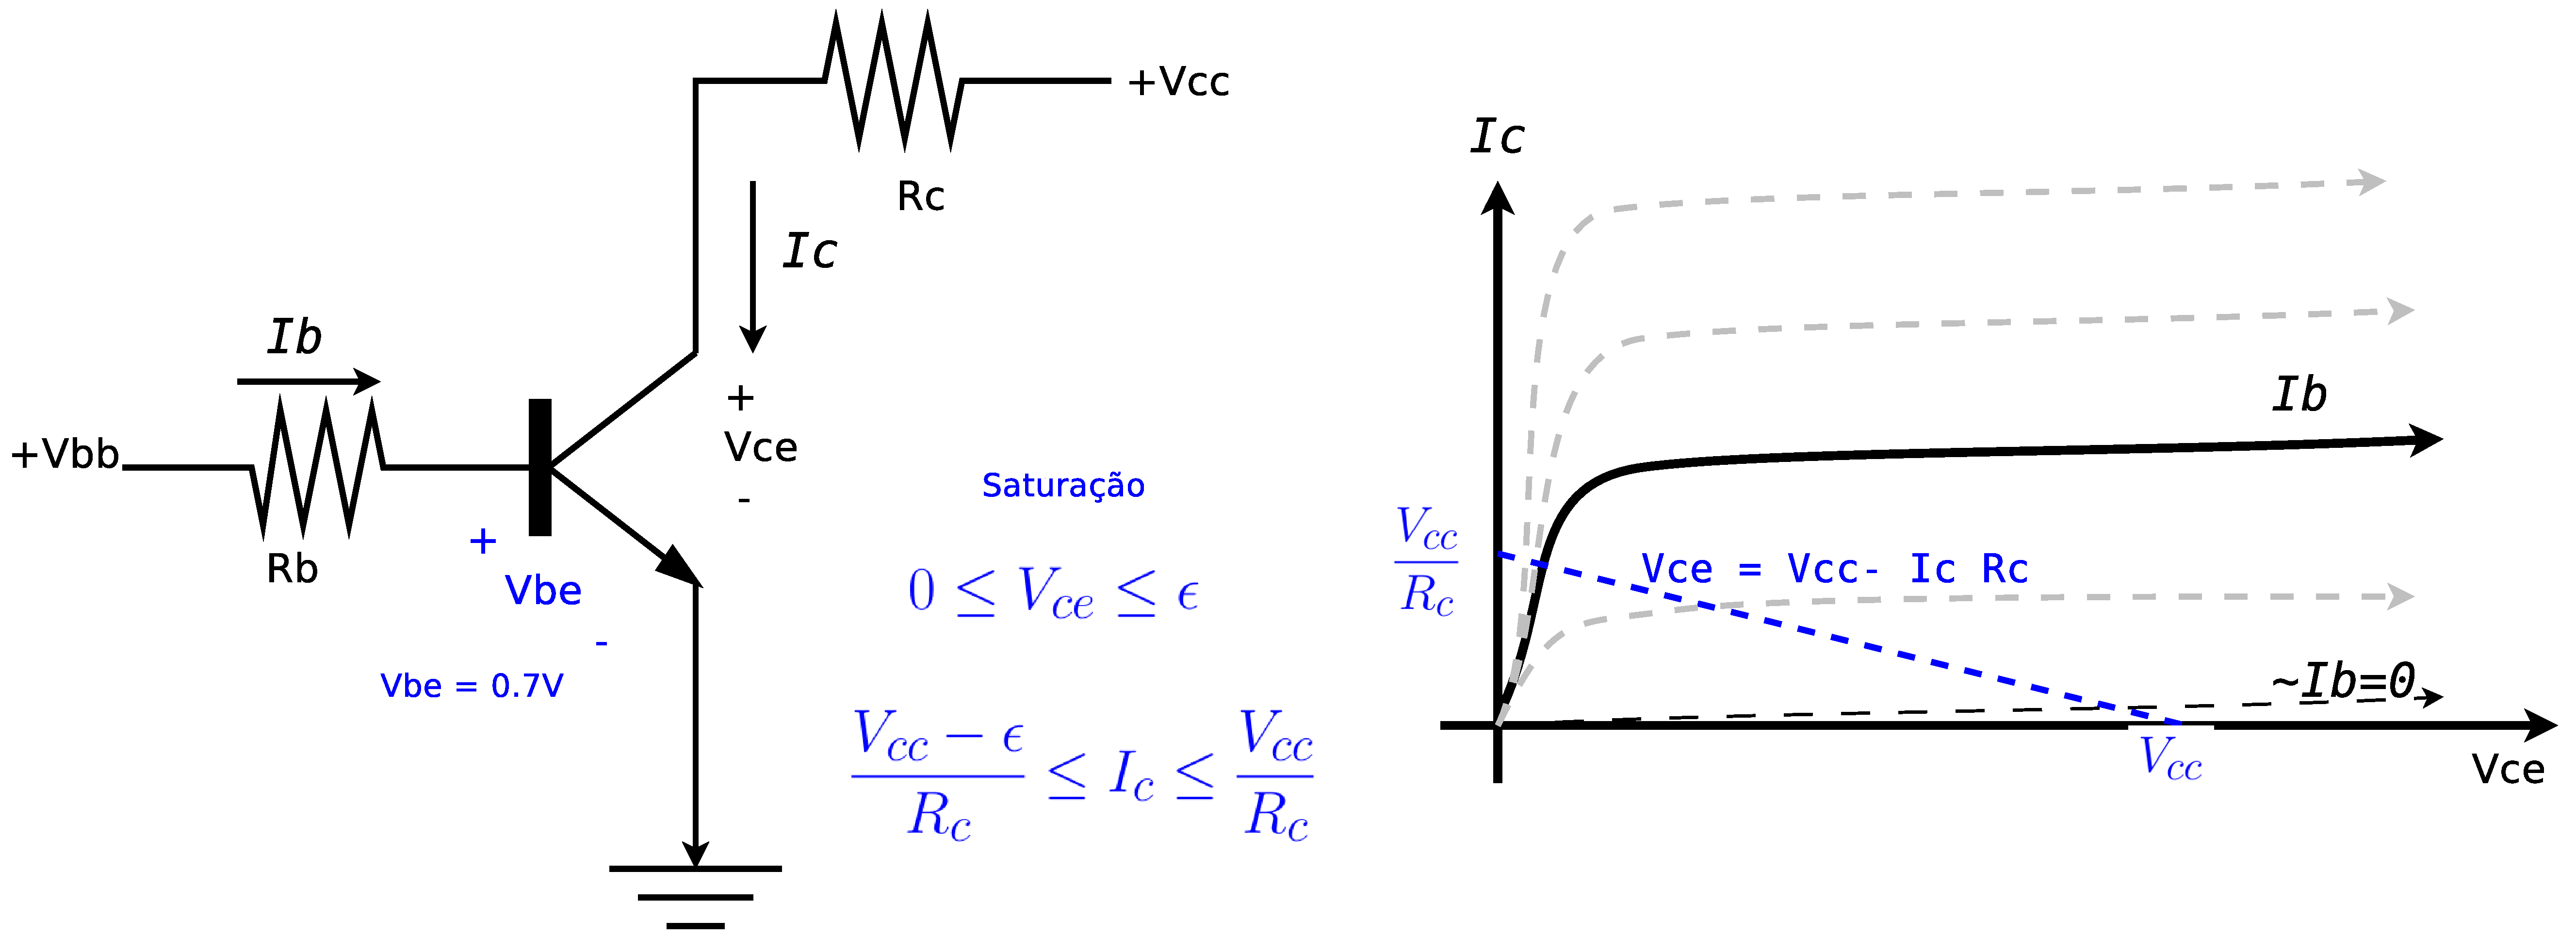
\includegraphics[width=10cm]{images/emisorcomun3.eps}
\caption{Transistor na região de saturação}
\label{fig:emisorcomun3}
\end{figure}
\end{frame}

%%%%%%%%%%%%%%%%%%%%%%%%%%%%%%%%%%%%%%%%%%%%%%%%%%%%%%%%%%%%%%%%%%%%%%%%%%%%%%%%
%%%%%%%%%%%%%%%%%%%%%%%%%%%%%%%%%%%%%%%%%%%%%%%%%%%%%%%%%%%%%%%%%%%%%%%%%%%%%%%%
%%%%%%%%%%%%%%%%%%%%%%%%%%%%%%%%%%%%%%%%%%%%%%%%%%%%%%%%%%%%%%%%%%%%%%%%%%%%%%%%
\begin{frame}{Exemplo de cálculo de valores de resistência}
\begin{figure}
\centering
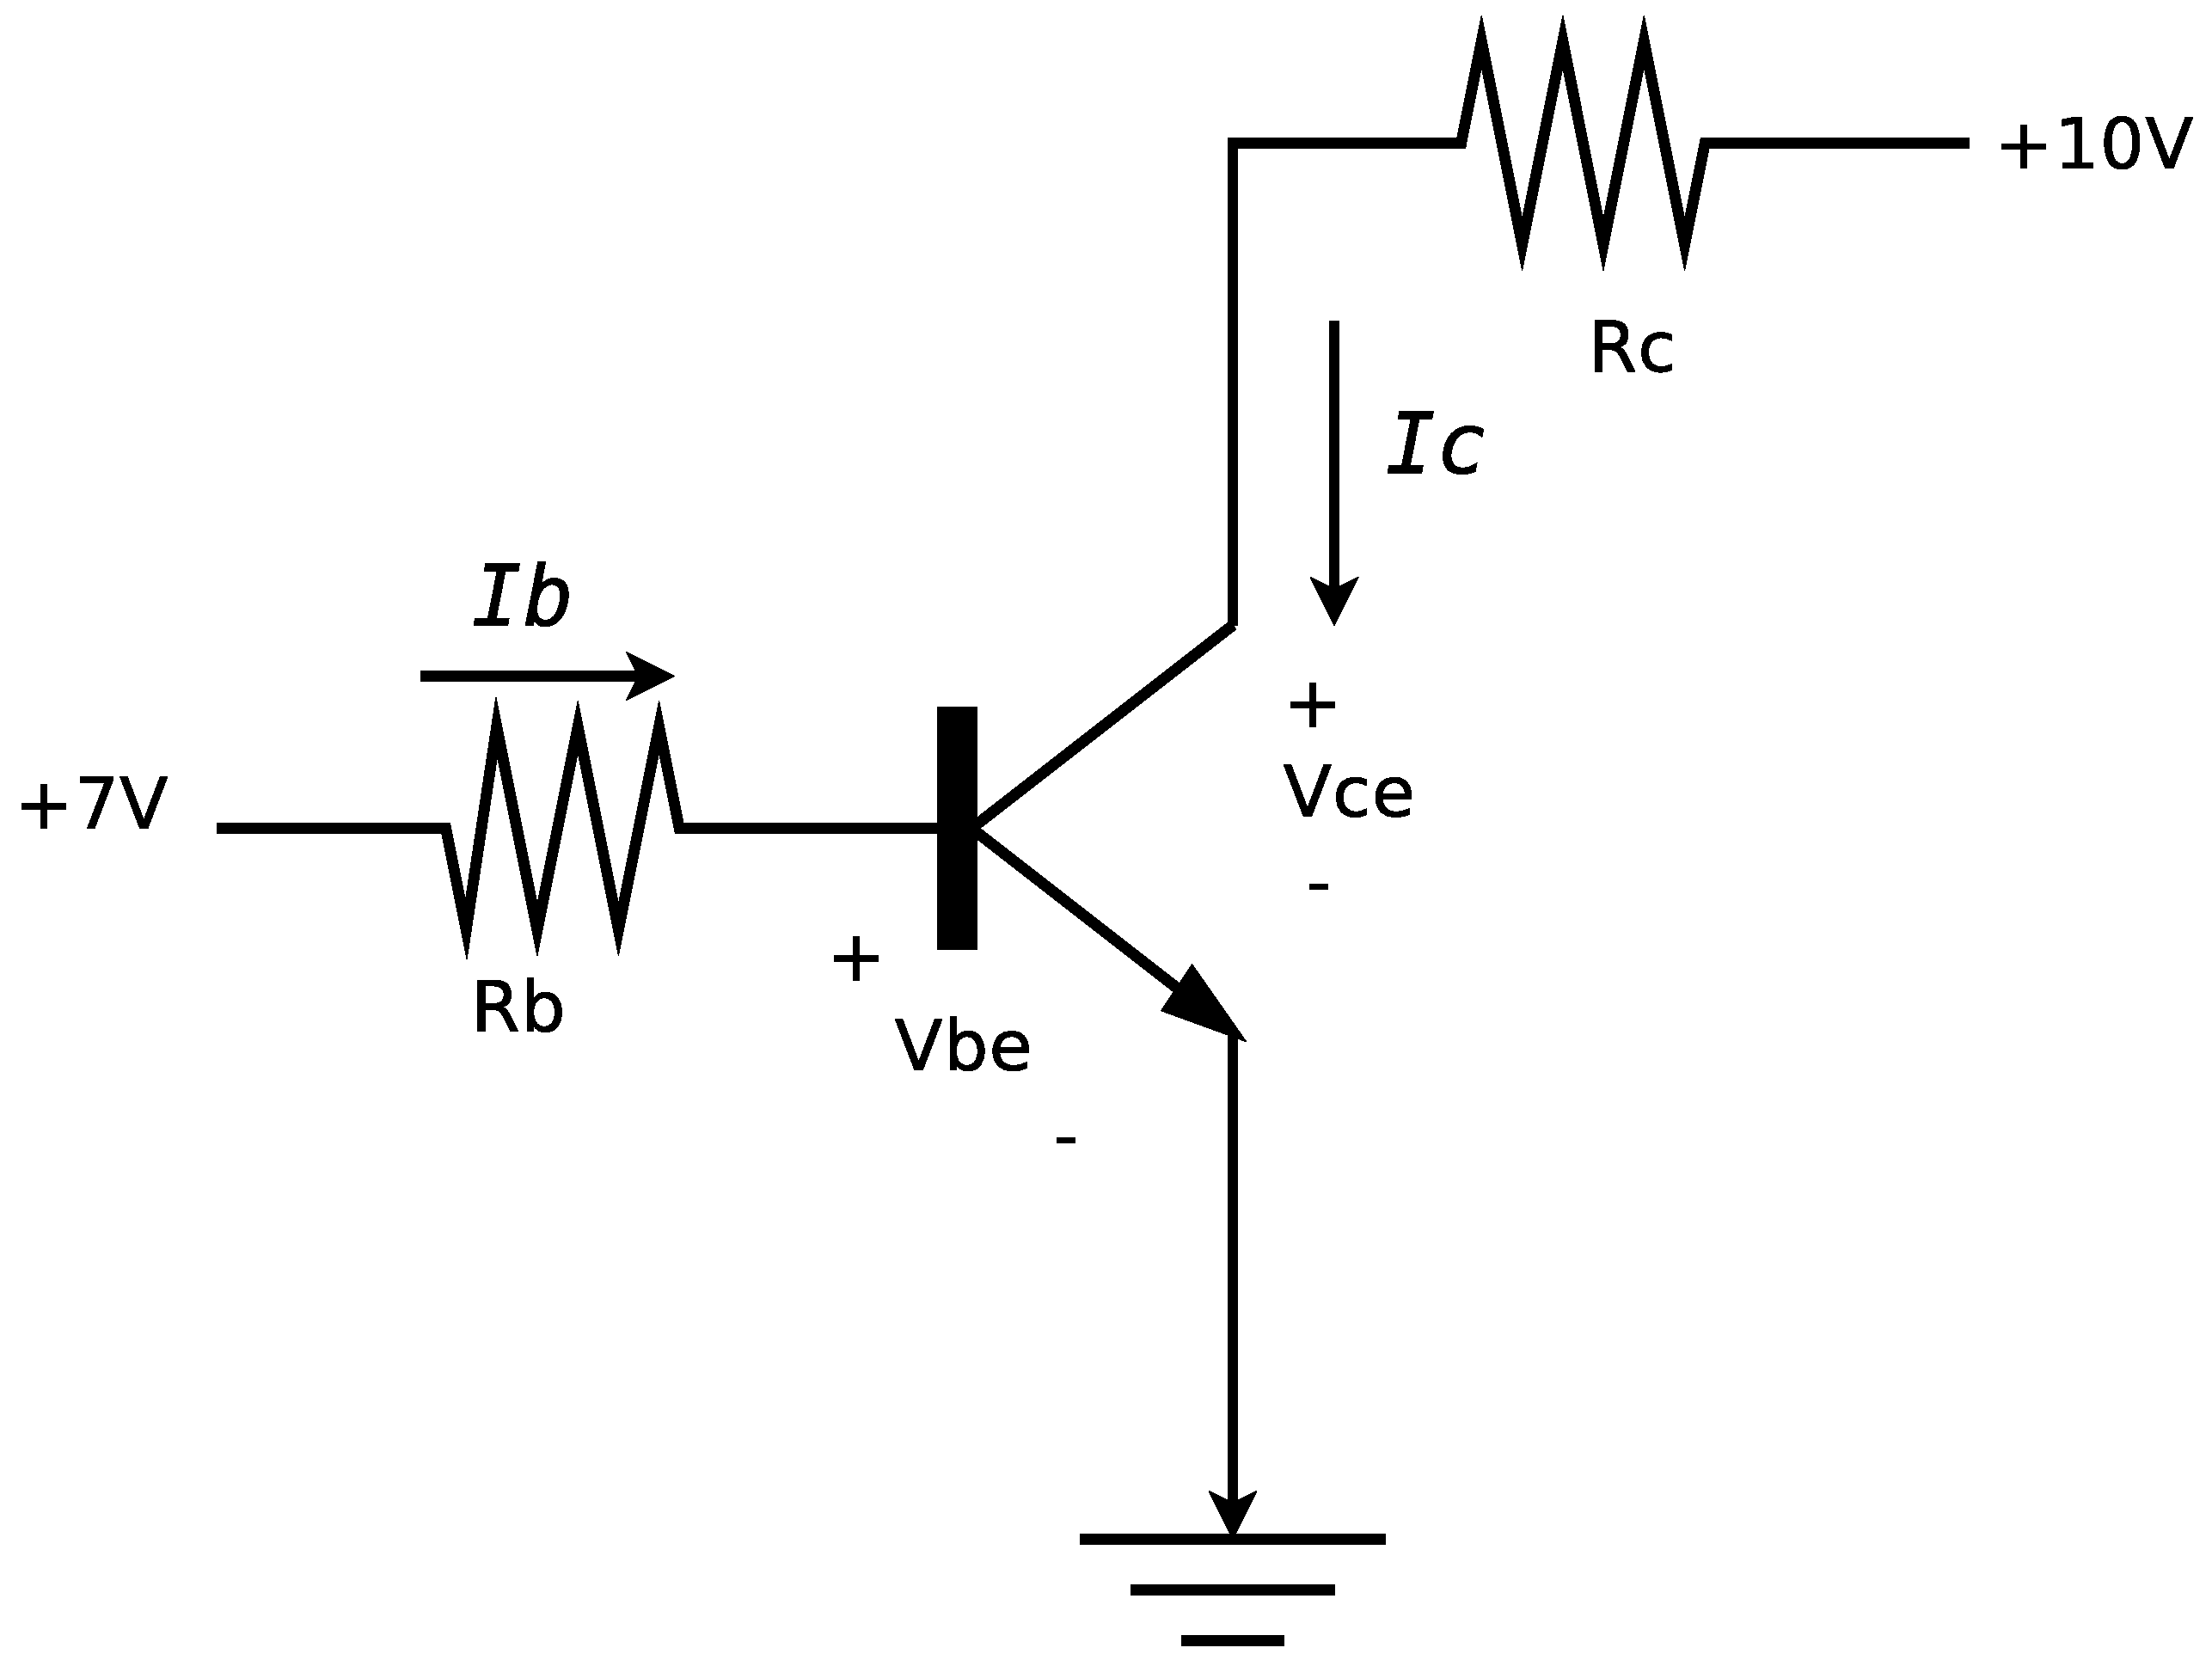
\includegraphics[width=7cm]{images/ejemplo1.eps}
\caption{Levar o transistor na região de corte}
\label{fig:ejemplo1a}
\end{figure}
\end{frame}

%%%%%%%%%%%%%%%%%%%%%%%%%%%%%%%%%%%%%%%%%%%%%%%%%%%%%%%%%%%%%%%%%%%%%%%%%%%%%%%%
\begin{frame}{Circuitos uteis}
\begin{figure}
\centering
\includegraphics[width=7cm]{images/espelhosimples.eps}
\caption{Espelho de corrente}
\label{fig:ejemplo1a}
\end{figure}
\end{frame}

%%%%%%%%%%%%%%%%%%%%%%%%%%%%%%%%%%%%%%%%%%%%%%%%%%%%%%%%%%%%%%%%%%%%%%%%%%%%%%%%
\begin{frame}[allowframebreaks]
        \frametitle{References}
        \bibliographystyle{plain}
\bibliography{transistor}
\end{frame}



\end{document}
